\documentclass[compress]{beamer} 

\usepackage[utf8]{inputenc}
\usepackage[brazil]{babel}
\usepackage{default}
\usepackage{setspace}

\usepackage{graphicx,url}
\usepackage{booktabs}
\usepackage{alltt}
\usepackage{xspace}
\usepackage{url}
\usepackage{amssymb}

\usepackage{caption}
\usepackage{moresize} %provides additional font sizes (HUGE and ssmall)
\usepackage{textcomp}
\usepackage{lmodern}
\usepackage{changepage}

\usepackage{animate}

\usepackage[ruled]{algorithm2e}
\SetKwBlock{When}{when}{end\_when}

\usepackage{xcolor}

\usepackage{minted}

\newcommand{\countasconf}{\langle  R_{e}, R_{s}, D, \mathcal{E}, \mathcal{N}, \mathcal{I},\mathcal{T}\rangle}
\newcommand{\jacamo}{$\mathsf{JaCaMo}$\xspace}
\newcommand{\moise}[0]{$\mathcal{M}$\textsc{oise}\xspace}
\newcommand{\cartago}{\textsf{CArtAgO}\xspace}
\newcommand{\Jason}{\textit{Jason}\xspace}

\newcommand{\sff}{\textit{status function}}
\newcommand{\sfs}{\textit{status functions}}
\newcommand{\Sfs}{\textit{Status functions}}
\newcommand{\crules}{\textit{constitutive rules}}
\newcommand{\Crules}{\textit{Constitutive rules}}
\newcommand{\crule}{\textit{constitutive rule}}

\newcommand{\shortminus}{\scalebox{0.3}[1.0]{$-$}} %a shorter minus signal

\newcommand{\cruleAlg}[4]{#1 \kwCountas #2 \\ \kwWhen #3 \\ \kwWhile #4}
\newcommand{\eg}[0]{\textcolor{blue}{e.g.}\xspace}

\captionsetup{labelformat=empty,labelsep=none}

\input{style-w}

%[Maiquel] *** commands for SAI spec. ***
\SetKw{kwCountas}{count-as}
\SetKw{kwWhen}{when}
\SetKw{kwWhile}{while}
\SetKw{kwStatusFunctions}{status\_functions}
\SetKw{kwCrules}{constitutive\_rules}
\SetKw{kwAgents}{agents}
\SetKw{kwEvents}{events}
\SetKw{kwStates}{states}
\SetKw{kwNorms}{norms}
\SetKw{kwObl}{obliged}
\SetKw{kwProhib}{prohibited}
\SetKw{kwPermitt}{permitted}
\SetKw{kwElse}{else}
\newcommand{\saicomment}[1]{\textcolor{olive}{/* #1 */}}

\newcommand{\yamlkey}[1]{\textcolor{red}{\texttt{#1}}}
\newcommand{\yamlvalue}[1]{\textcolor{blue}{\texttt{#1}}}



%http://latexcolor.com/
\definecolor{indiagreen}{rgb}{0.07, 0.53, 0.03}
\definecolor{harvestgold}{rgb}{0.85, 0.57, 0.0}
\definecolor{bulgarianrose}{rgb}{0.28, 0.02, 0.03}


\newcommand{\link}[2]{\href{#1}{\underline{\textcolor{blue}{#2}}}}

\newcommand{\planhead}[1]{\textcolor{indiagreen}{#1}}
\newcommand{\desire}[1]{\textcolor{blue}{#1}}
\newcommand{\instruction}[1]{\textcolor{red}{#1}}
\newcommand{\comment}[1]{\textcolor{harvestgold}{#1}}
\newcommand{\belief}[1]{\textcolor{violet}{#1}}
 
\title[]{Development of autonomous robots with \\ BDI agents and ROS
}
\author[]{{\bf Maiquel de Brito}}
\institute{%
\begin{minipage}[t]{.3\linewidth}\centering
\inst{1}UFSC-Blumenau-Brasil\\
\texttt{maiquel.b@ufsc.br}
\end{minipage}
%\and
%\begin{minipage}[t]{.3\linewidth}\centering
%\inst{2}FAYOL-EMSE, France\\
%\end{minipage}

}
\vspace{5.8cm}
%\date{{\scriptsize Florianópolis - Brazil \\ Sep. 2016}
%\begin{center}
	%\includegraphics[scale=0.1]{logo_ufsc.pdf}
	%\hfill
	%\raisebox{1.5mm}{\includegraphics[scale=0.4]{logo_ctc.pdf}}
	%\hfill
	%\raisebox{4mm}{\includegraphics[scale=0.3]{logoCapes.png}}
	%\end{center}
	%}
\date{
\begin{columns}
 \column{.2\textwidth}
 %\includegraphics[scale=0.1]{logo_ufsc.pdf}
 \column{.6\textwidth}
 \begin{center}
%  {\scriptsize 18th WESAAC}\\
%  {\scriptsize August 2024}
 \end{center}
 \column{.2\textwidth}
 
 %\includegraphics[scale=0.3]{logoCapes.png}
\end{columns}

}


%\titlegraphic{
%   \includegraphics[width=1cm]{logo_ufsc.pdf}\hspace*{6cm}
%   \includegraphics[width=.9cm]{logo_sepex}  
%   \includegraphics[width=3cm]{logo-arc6-72dpi.jpg}
%}


\begin{document}

\begin{frame}[plain]
  \titlepage
\end{frame}


%\begin{frame}{Outline}
%  \scriptsize
%  \tableofcontents
%\end{frame}

\begin{frame}{Preliminaries}
 
    {\bf What are we going to see in this course?}
    \begin{itemize}\scriptsize
        \item Programming ROS-based robots controlled by Jason agents
        \item Essentials on Jason and ROS
    \end{itemize}
    
    
    \vspace{1cm}
    
    {\bf What are we not going to see in this course?}
    \begin{itemize}\scriptsize
     \item Details on ROS
     \item Details on Jason
    \end{itemize}

    
    \vfill
    
 {\tiny Practical activities are available \link{https://github.com/embedded-mas/jason-ros-course-wesaac2024/blob/main/README.adoc}{here}} 

 
 
\end{frame}

\begin{frame}
 

 \HUGE
\centering
--- Part I ---\\
ROS 
 
\end{frame}



\section{Part I - Introduction to ROS}

\begin{frame}{What is ROS?}
    %\begin{itemize}
        \textbf{ROS --- Robot Operating System}: \\ A flexible framework for writing robot software\\
        
        %\vspace{.35cm}
        \footnotesize
        Provides tools and libraries to help developers to create robot applications\\
        
        \vspace{.5cm}
        \textbf{Key Components:}
        \begin{itemize}
            \item \textbf{Middleware}: For inter-process communication and hardware abstraction
            \item \textbf{Tools}: For development, debugging, and visualization.
            \item \textbf{Ecosystem}: Large community and a vast repository of packages.
        \end{itemize}
    %\end{itemize}
\end{frame}



\begin{frame}{The Turtlesim simulation}

\footnotesize

The hands on part of this course uses the well-known \link{http://wiki.ros.org/turtlesim}{turtlesim} simulator\\
{\tiny with some extensions}

\vspace{.5cm}

\scriptsize

\begin{columns}
 \column{.55\textwidth}
 One or more turtle-shaped robots in a square world\\
{\tiny whose sensors and actuators are controlled by ROS}\\ \vspace{.5cm}
 The robots can freely move and leave a trail wherever they go
 \vspace{.5cm}
 
 Positions in the environment follow the cartesian coordinate system \\ \tiny{being thus given by the coordinates $(x,y)$}
 
 \hspace{-20pt} % Adjust space between columns
 
 \column{.35\textwidth}
  \begin{figure}
   \centering
   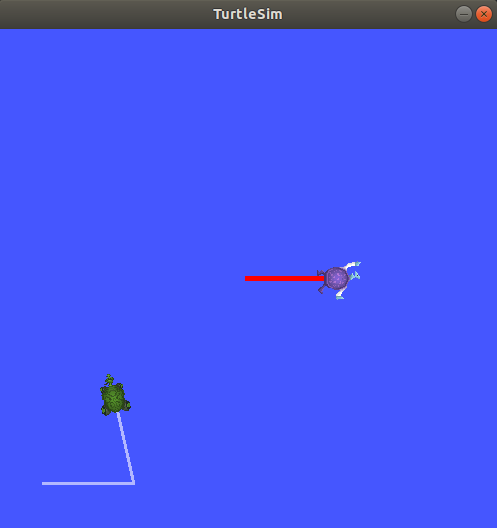
\includegraphics[width=.9\textwidth]{turtlesim.png}
    % turtlesim.png: 497x528 px, 72dpi, 17.53x18.63 cm, bb=0 0 497 528
    %\caption{source: \href{docs.ros.org/en/foxy/_images/remap.png}}
  \end{figure}
\end{columns}


\vfill
{\tiny Go to the Preliminaries -- Running ROS section of the \link{https://github.com/embedded-mas/jason-ros-course-wesaac2024}{tutorial}}
\end{frame}


\subsubsection{ROS Architecture}

\begin{frame}{ROS Architecture}
    %\begin{columns}
        %\column{0.5\textwidth}
        %\begin{itemize} 
        
            \textbf{Nodes}: Processes that perform computation.\\   \vspace{.1cm}
            
            \textbf{Topics}: Named buses for asynchronous communication.\\ \vspace{.1cm}
            
            
            \textbf{Services}: Synchronous remote procedure calls.\\ \vspace{.1cm}
            
            
            \textbf{Messages}: Data structures for communication.\\ \vspace{.1cm}
            
            %\textbf{Bags}: For recording and playback of messages.\\ \vspace{.1cm}
            
            \vfill
            
            {\tiny \href{https://miro.medium.com/v2/format:webp/0*n7FfmKCTMjXgD7_V.gif}{\underline{\textcolor{blue}{ROS architecture scheme}}}}
        %\end{itemize}
        %\column{0.5\textwidth}
        %\animategraphics[loop,width=\textwidth]{ros_arch.gif} % Replace with your image path
        %https://medium.com/software-architecture-foundations/robot-operating-system-2-ros-2-architecture-731ef1867776
    %\end{columns}
\end{frame}

\begin{frame}{ROS Nodes}

   \footnotesize

   Processes that perform computation.\\  
   {\tiny the smallest executable unit of ROS -- either Python scripts or C++ compiled files}
   
   \vspace{0.5cm}
   
   
   
   Responsible for a single, modular purpose\\
   {\tiny e.g. one node for controlling wheel motors, one node for controlling a laser range-finder, etc.} 
   
   \vspace{0.5cm}
   
   
  \footnotesize
   
   Can interact with each other {\tiny even running in different machines}\\
   following some interaction pattern:\\
   \vspace{-.5cm}
   \begin{itemize}\ssmall
    \item publish/subscribe (topics)
    \item client/server (services)
    \item action client/action server (actions)
   \end{itemize}

   
   \vspace{.5cm}
   
   Launching a node:   \texttt{ros2 run <package name> <node name>}\\

   
    \vfill
    {\fontsize{4}{4.8}\selectfont more on ROS nodes \href{https://docs.ros.org/en/foxy/Tutorials/Beginner-CLI-Tools/Understanding-ROS2-Nodes/Understanding-ROS2-Nodes.html}{\textcolor{blue}{\underline{here}}}}
 
   
\end{frame}

\begin{frame}{ROS Topics}

  \footnotesize

  Topics are data containers\\ \vspace{.2cm}
  
  Nodes may 
  \begin{itemize}
   \item publish data to any number of topics \\ {\tiny multiple nodes can publish data to the same topic}
   \item subscribe to any number of topics\\ {\tiny subscribers are updated when the topic data changes}
  \end{itemize}

  
  %\vspace{.5cm}
  {\tiny \href{https://docs.ros.org/en/crystal/_images/Topic-MultiplePublisherandMultipleSubscriber.gif}{\underline{\textcolor{blue}{ROS topic illustration}}}}
  
  \vspace{.25cm}
  
  \begin{block}{{\tiny useful command line topic tools}}\tiny
    List of available topics: \texttt{ros2 topic list}\\
    Publish on a topic: \texttt{ros2 topic pub \textless topic name\textgreater\ \textless msg type\textgreater\  \textless content\textgreater }\\
    Listen to topic updates: \texttt{ros2 topic echo \textless topic name\textgreater\ }\\
    Get information about the topic: \texttt{ros2 topic info \textless topic name\textgreater\ }
   
  \end{block}

 
 \vfill
{\fontsize{4}{4.8}\selectfont more on ROS topics \link{https://docs.ros.org/en/foxy/Tutorials/Beginner-CLI-Tools/Understanding-ROS2-Topics/Understanding-ROS2-Topics.html}{here}}
 
\end{frame}


\begin{frame}{ROS Messages}

  \footnotesize
 
 Messages describe the data structures \\ {\ssmall that record the information to be exchanged among the nodes}\\%\vspace{.5cm}
 
 Composed of fields that have a name and a type \\ 
 
 %\vspace{.5cm}
 
 A type may be either another message or a primitive type\\
 {\tiny examples of primitive types: \texttt{bool}, \texttt{int32}, \texttt{float64}}\\
 
 
 Checking the message structure: \texttt{ros2 interface show \textless message type\textgreater\ }
 
 \vspace{.25cm}
 \begin{block}{{\ssmall Examples}}
 \ssmall
 \begin{columns}
  \column{.25\textwidth}
  \texttt{std\_msgs/msg/Float64}\\
  \texttt{\ \ \ float64 data} \\
  \ \\
  \ \\
  \column{.25\textwidth}
  \texttt{geometry\_msgs/Vector3}\\
  \texttt{\ \ \ float64 x\\
          \ \ \ float64 y\\
          \ \ \ float64 z}
  
  \column{.33\textwidth}
  \texttt{geometry\_msgs/msg/Twist}\\
  \texttt{\ \ \ Vector3  linear\\  
   \ \ \ Vector3  angular}\\
\ \\

 \end{columns}
\end{block}

{\tiny Go to exercises 1.1.1 and 1.1.2}

\vfill

{\fontsize{4}{4.8}\selectfont more on ROS messages \link{https://docs.ros.org/en/foxy/Concepts/About-ROS-Interfaces.html}{here}}
\end{frame}



\begin{frame}{The Turtlesim simulation}
\framesubtitle{{\bf Subscribed topics}}
\footnotesize
 \texttt{turtleX/cmd\_vel [geometry\_msgs/msg/Twist]}\\ \vspace{.2cm}
 
Records the intended linear and angular velocity of the robot\\ \vspace{.1cm}

The robot controller reads the topic and adjusts its velocity accordingly\\
{\tiny keeping the velocity for 1 second}\\
 
 
 \vspace{.2cm}
 \begin{block}{{\tiny geometry\_msgs/msg/Twist}}
 \begin{columns}
   
    
  \column{.24\textwidth}
    %\begin{block}{{\tiny geometry\_msgs/msg/Twist}}
       \tiny
         \begin{alltt}
            Vector3  linear\\
            \ \ \ \ \ \ \ \ float64 x\\
            \ \ \ \ \ \ \ \ float64 y\\
            \ \ \ \ \ \ \ \ float64 z\\
            Vector3  angular\\
            \ \ \ \ \ \ \ \ float64 x\\
            \ \ \ \ \ \ \ \ float64 y\\
            \ \ \ \ \ \ \ \ float64 z\\
            \ \\            
        \end{alltt}
    %\end{block}
     \column{.65\textwidth}
     \tiny
     \texttt{linear.x}: controls the forward ($x>0$) and backward ($x<0$) movement\\ \vspace{.1cm}
     \texttt{linear.y}: controls the upward ($y>0$)  and  downward ($y<0$) movement\\ \vspace{.1cm}
     \texttt{linear.z}: no effect in turtlesim\\ \vspace{.1cm}
     \texttt{angular.x}: no effect in turtlesim\\ \vspace{.1cm}
     \texttt{angular.y}: no effect in turtlesim\\ \vspace{.1cm}
     \texttt{angular.z}: controls the clockwise ($z<0$) and counterclockwise ($z>0$) \\ \ \ \ \ \ \ \ \ \ \ \ \ \ \ \ \ movement around the robot's axis
 \end{columns}
 \end{block}
\end{frame}



\begin{frame}{The Turtlesim simulation}
\framesubtitle{{\bf Published topics}}
\footnotesize
 \texttt{/turtle1/pose [turtlesim/msg/Pose]}\\ \vspace{.5cm}
 
 Records the robot's position, angle, and linear and angular velocity\\
 {\tiny the robot updates this topic when these values change.}
 
 
 \vspace{.5cm}
 \begin{block}{{\tiny turtlesim/msg/Pose}}
 \begin{columns}
   
    
  \column{.24\textwidth}
       \tiny
         \begin{alltt}
            float32 x\\
            float32 y\\
            float32 theta\\    
            float32 linear\_velocity \\
            float32 angular\_velocity\\
            \ \\
            \ \\ 
        \end{alltt}
     \column{.65\textwidth}
     \tiny
     \texttt{x}: position of the robot in the x axis\\ \vspace{.1cm}
     \texttt{y}: position of the robot in the y axis\\ \vspace{.1cm}
     \texttt{theta}: angle of the robot with respec to the x axis\\ \vspace{.1cm}
     \texttt{linear\_velocity}: linear velocity of the robot\\ \vspace{.1cm}
     \texttt{angular\_velocity}: linear velocity of the robot
 \end{columns}
 \end{block}
 
 
 \vfill 
 
 {\tiny Go to exercise 1.1.3}  
 
 
\end{frame}




\begin{frame}{ROS Services}
 
 \footnotesize
 
 Services are functions provided by the nodes\\
 {\tiny to be requested by other nodes following a client/server pattern with blocking communication}\\
 
 
 May return some information as result of the execution\\ 
 
 Services have a \textit{type} that defines the \textit{message type} of both the request and response
 
 \vspace{.5cm}
 
   \begin{block}{{\tiny useful command line topic tools}}\tiny
    List of available services: \texttt{ros2 service list}\\
    Call a service: \texttt{ros2 service call \textless service name\textgreater\ \textless service args\textgreater\ }\\
    Get the service type: \texttt{ros2 service type \textless service name\textgreater\ }
   
  \end{block}

{\tiny Go to exercises 1.2.1 and 1.2.2}  
 
 \vfill
{\fontsize{4}{4.8}\selectfont more on ROS services \link{https://docs.ros.org/en/foxy/Tutorials/Beginner-CLI-Tools/Understanding-ROS2-Services/Understanding-ROS2-Services.html}{here}}
 
\end{frame}





\begin{frame}{The Turtlesim simulation}
\framesubtitle{{\bf Provided Services}}
\footnotesize
 \texttt{/turtle1/teleport\_absolute [turtlesim/srv/TeleportAbsolute]}\\ \vspace{.5cm}
 
 Moves the robot's to a given point $(x,y)$ in the environment \\
 {\tiny and rotates the robot if needed}
 
 
 \vspace{.5cm}
 \begin{block}{{\tiny turtlesim/srv/TeleportAbsolute}}
 \begin{columns}
   
    
  \column{.24\textwidth}
       \tiny
         \begin{alltt}
            float32 x\\
            float32 y\\
            float32 theta\\
            \ \\
            \ \\
        \end{alltt}
     \column{.65\textwidth}
     \tiny
     \texttt{x}: target position in the x axis\\ \vspace{.1cm}
     \texttt{y}: target position in the y axis\\ \vspace{.1cm}
     \texttt{theta}: target angle with respec to the x axis\\
     {\tiny \ \ \ \ \ \ \ \ \ \ in radians }
     {\tiny $\alpha_{rad}=\frac{\alpha^{\circ}\times \pi}{180}$}
 \end{columns}
 \end{block}
 
 
\vfill 
 
{\tiny Go to exercice 1.2.3} 
 
\end{frame}





\begin{frame}{The Turtlesim simulation}
\framesubtitle{{\bf Provided Services}}
\footnotesize
 \texttt{/turtle1/teleport\_Relative [turtlesim/srv/TeleportRelative]}\\ \vspace{.5cm}
 
 Moves the robot's along a given distance forward/backward \\
 {\tiny and rotates the robot if needed}
 
 
 \vspace{.5cm}
 \begin{block}{{\tiny turtlesim/srv/TeleportRelative}}
 \begin{columns}
   
    
  \column{.24\textwidth}
       \tiny
         \begin{alltt}
            float32 linear\\
            float32 angular\\
            \ \\
            \ \\
        \end{alltt}
     \column{.65\textwidth}
     \tiny
     \texttt{linear}: distance to move the robot forward/backward\\ \vspace{.1cm}
     \texttt{angular}: angle to rotate the robot\\ 
     {\tiny \ \ \ \ \ \ \ \ \ \ \ \ \ in radians }
     {\tiny $\alpha_{rad}=\frac{\alpha^{\circ}\times \pi}{180}$}
 \end{columns}
 \end{block}
 
 \vfill 
 
{\tiny Go to exercices 1.2.4 and 1.2.5}
 
\end{frame}


\section{Part II - Introduction to Jason}



\begin{frame}
 

 \HUGE
\centering
--- Part II ---\\
BDI Agents\\
Jason
 
\end{frame}


\begin{frame}{What is an agent?}

\begin{figure}[htbp]

\scriptsize

\textit{``... anything ... perceiving its environment through sensors and acting upon that environment through actuators''}{\tiny \cite{russel1995}}

\vspace{.5cm}

\textit{``... a computer system that is situated in some environment, and that is capable of
autonomous action in this environment in order to meet its delegated objectives..''}{\tiny \cite{wooldridge2009}}\\




 \centering
 
 \begin{figure}
 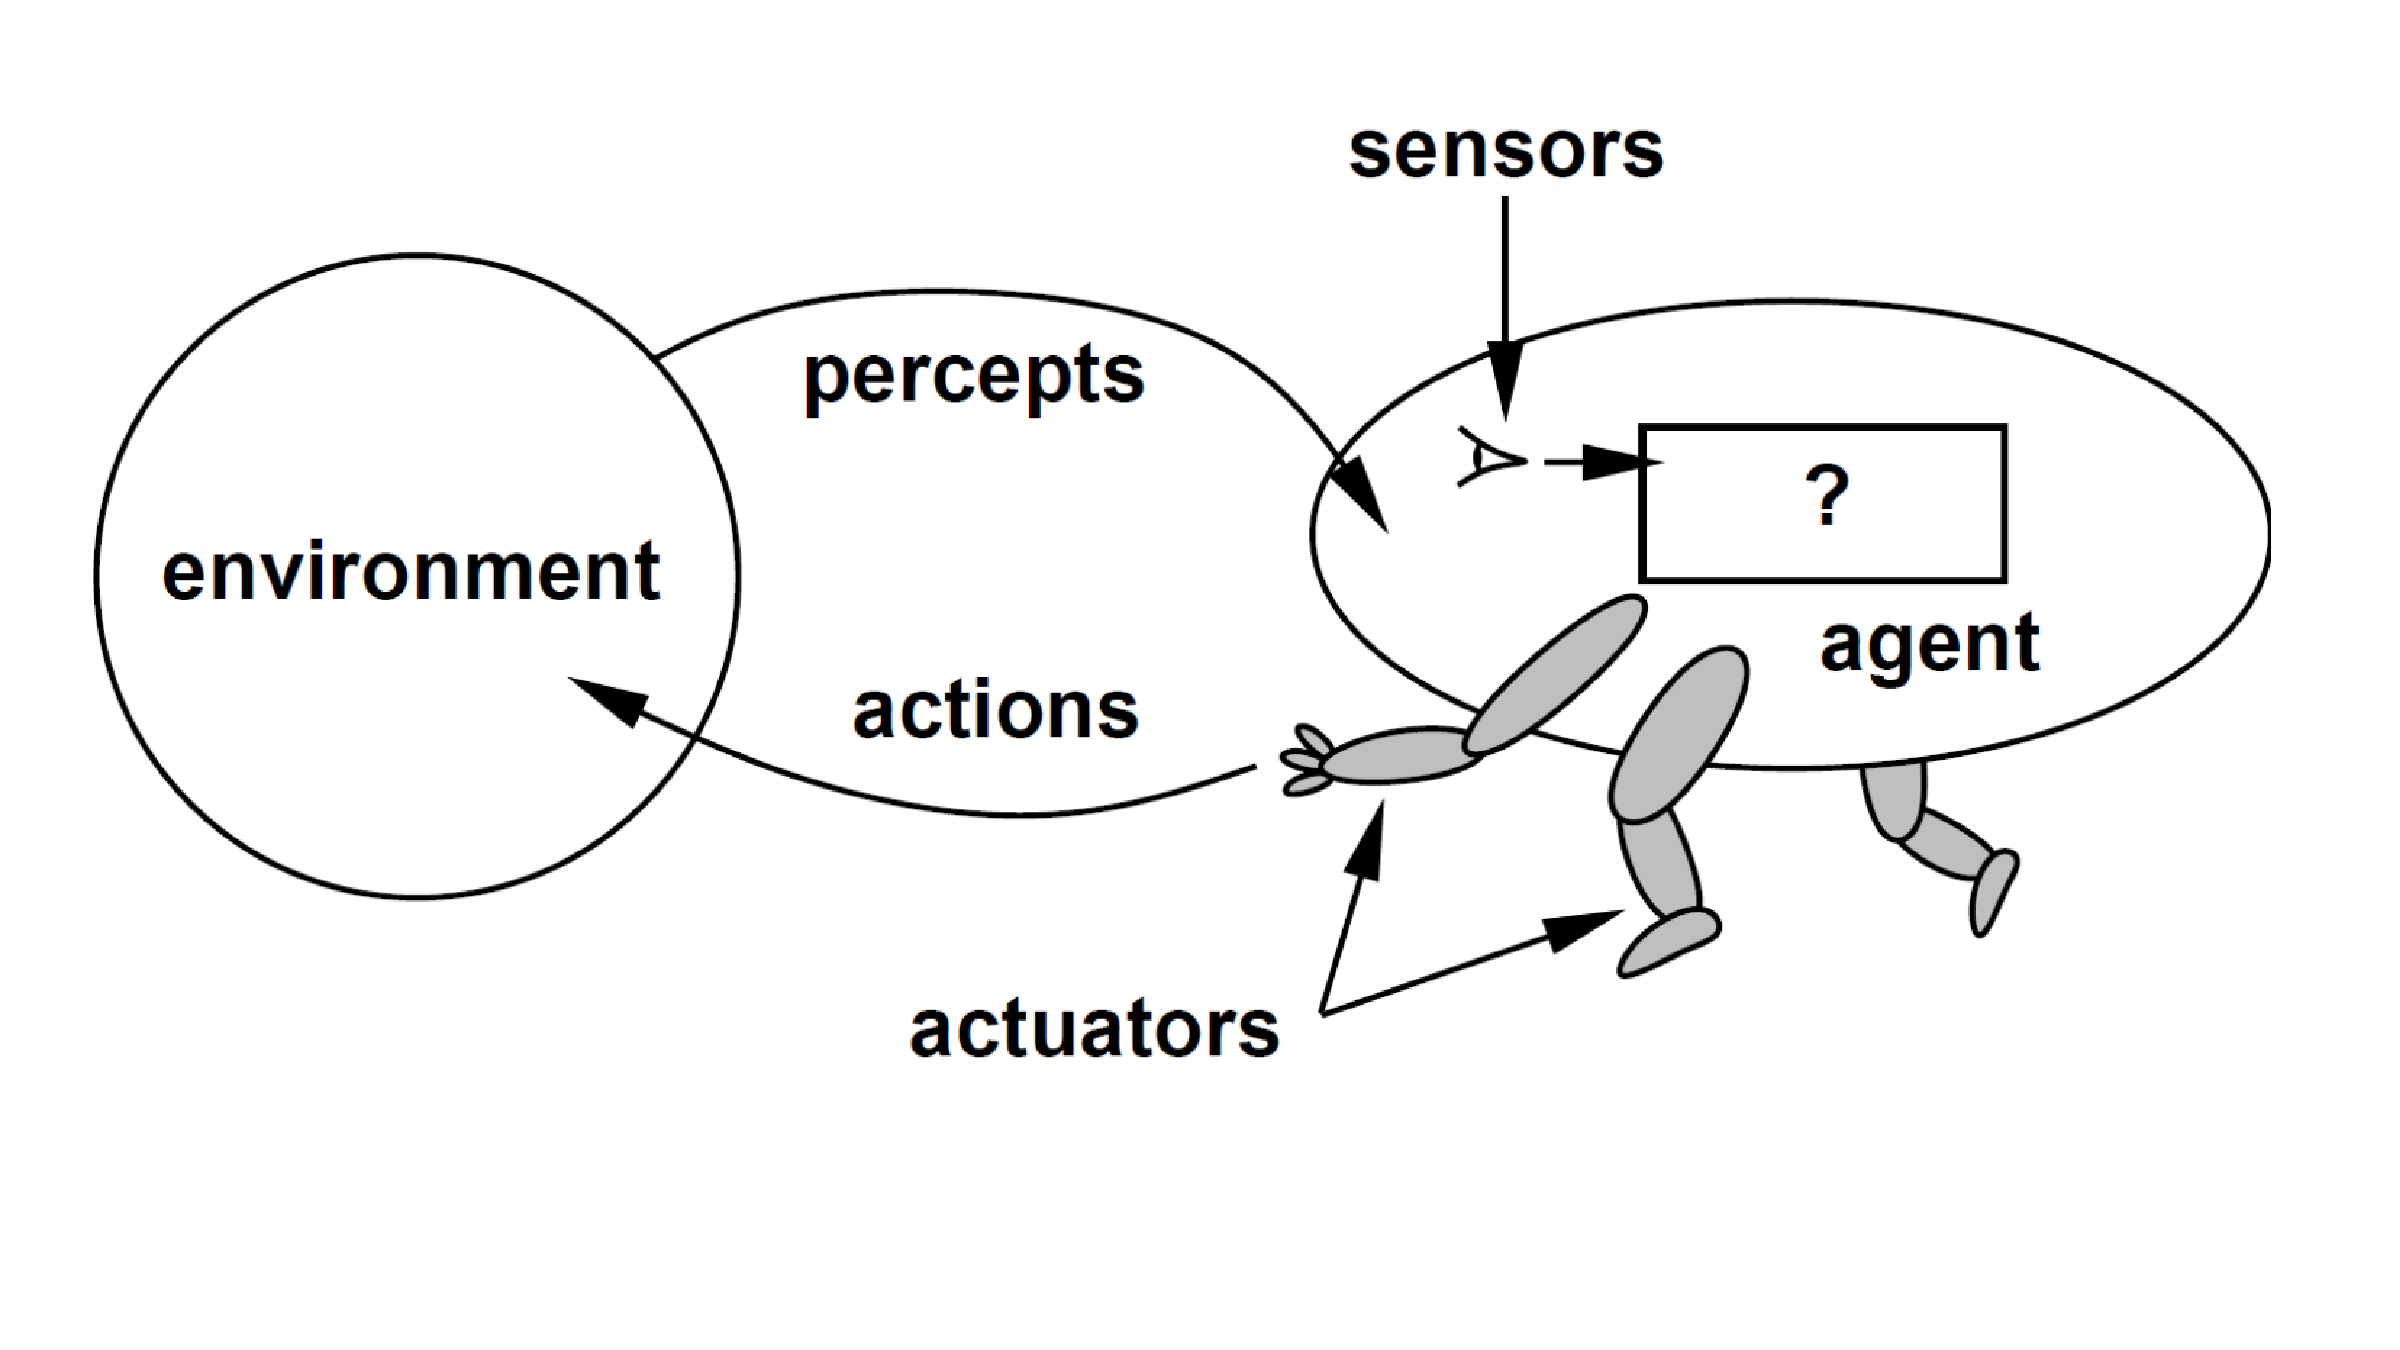
\includegraphics[scale=.15]{agent-russel-norvig.pdf}
  \caption{{\tiny Image from~\cite{russel1995}}}
 \end{figure}
\end{figure}

 
\end{frame}


\begin{frame}{The BDI Architecture}

{\bf B}eliefs, {\bf D}esires, and {\bf I}ntentions\\ \vspace{1cm}

{\bf Beliefs}\\
\footnotesize
\ \ \ Information that the agent possesses about the world in which it operates\\

\vspace{.5cm}
{\bf Desires}\\
\footnotesize
\ \ \ States of the world that the agent would like to achieve (\textit{options})\\

\vspace{.5cm}
{\bf Intentions}\\
\footnotesize
\ \ \ States of the world that the agent has decided to act upon to achieve

\end{frame}


\begin{frame}{The BDI Architecture}

\footnotesize

\begin{block}{{\scriptsize Example: autonomous vehicle}}
\scriptsize

Beliefs: current position, current speed, available energy\\ \vspace{.2cm}

Desires: reach the destination quickly, maintain energy above a certain threshold \\ \vspace{.2cm}

Intentions: if energy falls below the threshold: acquire energy\\ \vspace{.2cm}

\end{block}



\end{frame}



\begin{frame}{The BDI Architecture}

How does an agent go from its BDI to actions?\\ \vspace{.5cm}

{\bf Practical Reasoning}\\

\vspace{-.2cm}

\ \ \ Deciding among options {\tiny (based on its knowledge)}\\

\vspace{-.5cm}

\ \ \ {\footnotesize which can even be conflicting} {\tiny (e.g., reach the destination quickly vs. maintain energy)}\\

%\vspace{1cm}

{\bf Practical Reasoning Involves Two Processes}\\ \vspace{-.2cm}
\begin{enumerate}\footnotesize
 \item \textit{Deliberation}: deciding which intentions to adopt \vspace{.2cm}
 \item \textit{Means-End Reasoning}: deciding the sequence of actions to follow\\ 
 to satisfy the adopted intentions
\end{enumerate}

\end{frame}


\begin{frame}{The BDI Architecture}

How does a BDI computer program behave?
\begin{columns}
 \column{.5\textwidth}
  \begin{enumerate}\scriptsize
   \item Perceives the world and updates beliefs\vspace{.3cm}
   \item Evaluates its desires and decides which intention(s) to achieve\vspace{.3cm}
   \item Through means-end reasoning, defines a plan to satisfy the intention\vspace{.3cm}
   \item Executes the plan
  \end{enumerate}

 \column{.5\textwidth}
 
 \begin{figure}[htbp]
 \centering
 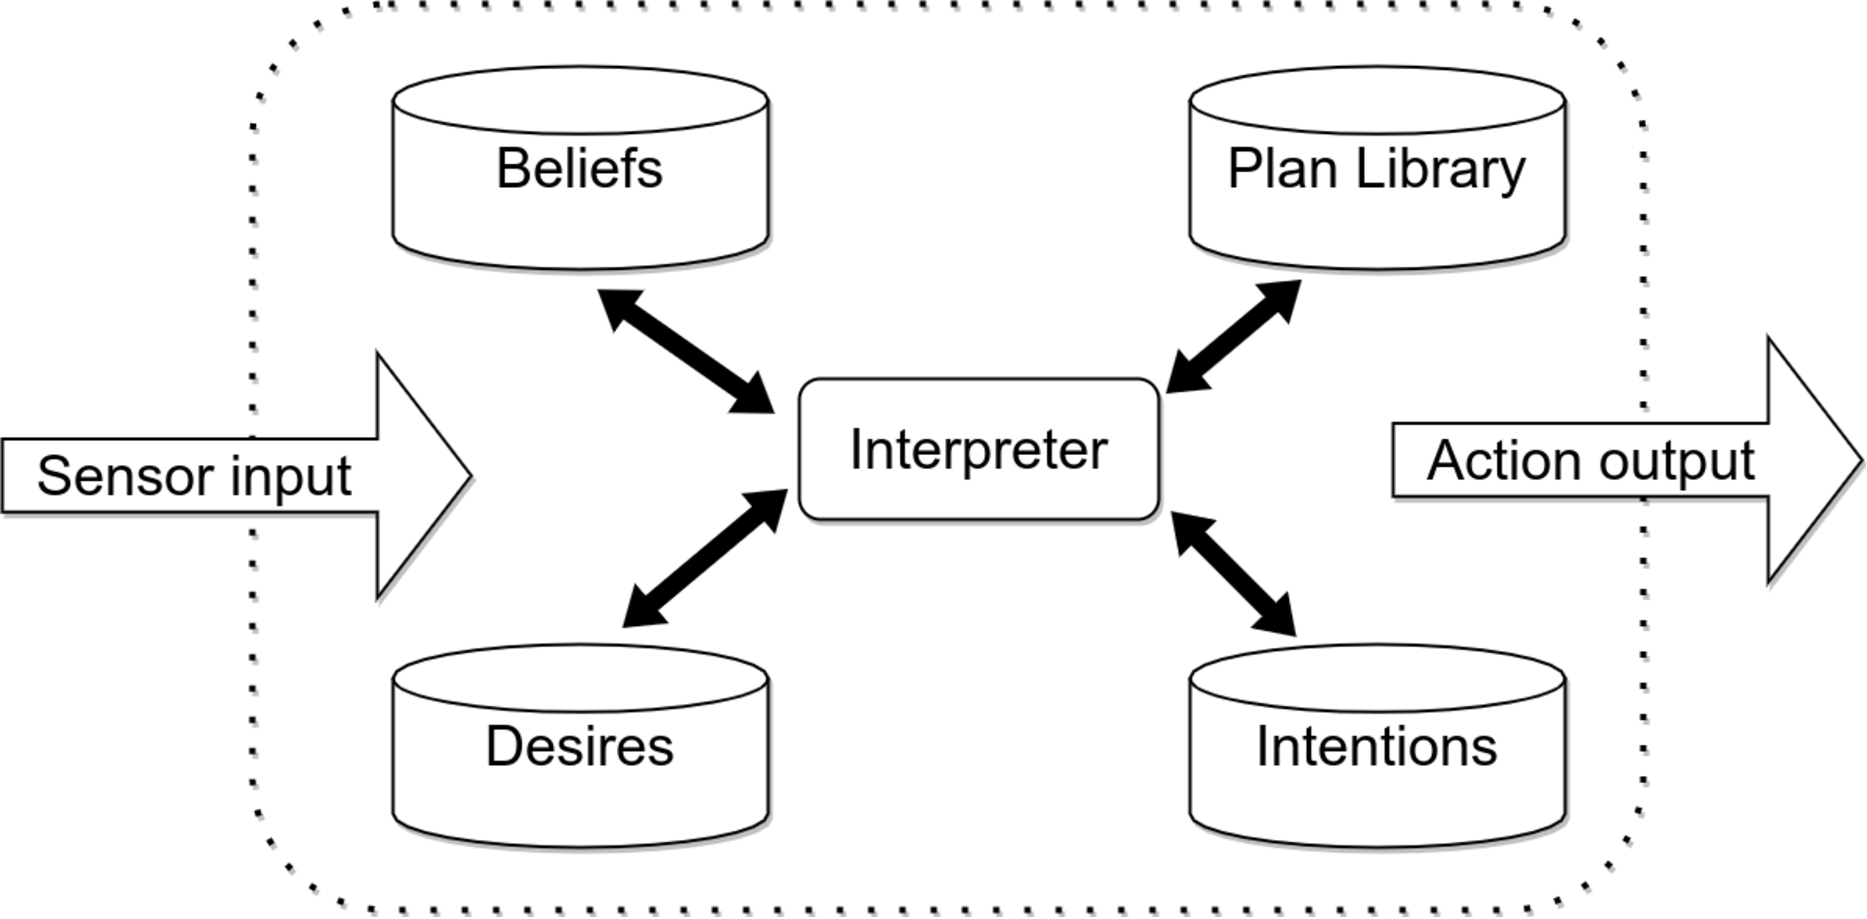
\includegraphics[scale=0.18]{BDI.pdf}
 % bdi1.pdf: 0x0 px, 300dpi, 0.00x0.00 cm, bb=
 \caption{{\tiny Adapted from \cite{bordini2007}}}
\end{figure}
\end{columns}

\end{frame}

\begin{frame}{How to Implement BDI?}

 How to implement programs with BDI behavior?\\
 
 %\vspace{.5cm}
 
 It is necessary to implement:
 \begin{columns}
 \column{.5\textwidth}
  \begin{enumerate}\scriptsize
   \item perception mechanisms
   \item representation of beliefs, desires, plans
   \item belief revision
   \item generation of intentions
   \item deliberation
   \item means-end reasoning
   \item communication mechanisms
   \item plan execution mechanisms
   \item etc, etc, etc...
   \item agent behavior
  \end{enumerate}

 \column{.5\textwidth}
 
 \begin{figure}[htbp]
 \centering
 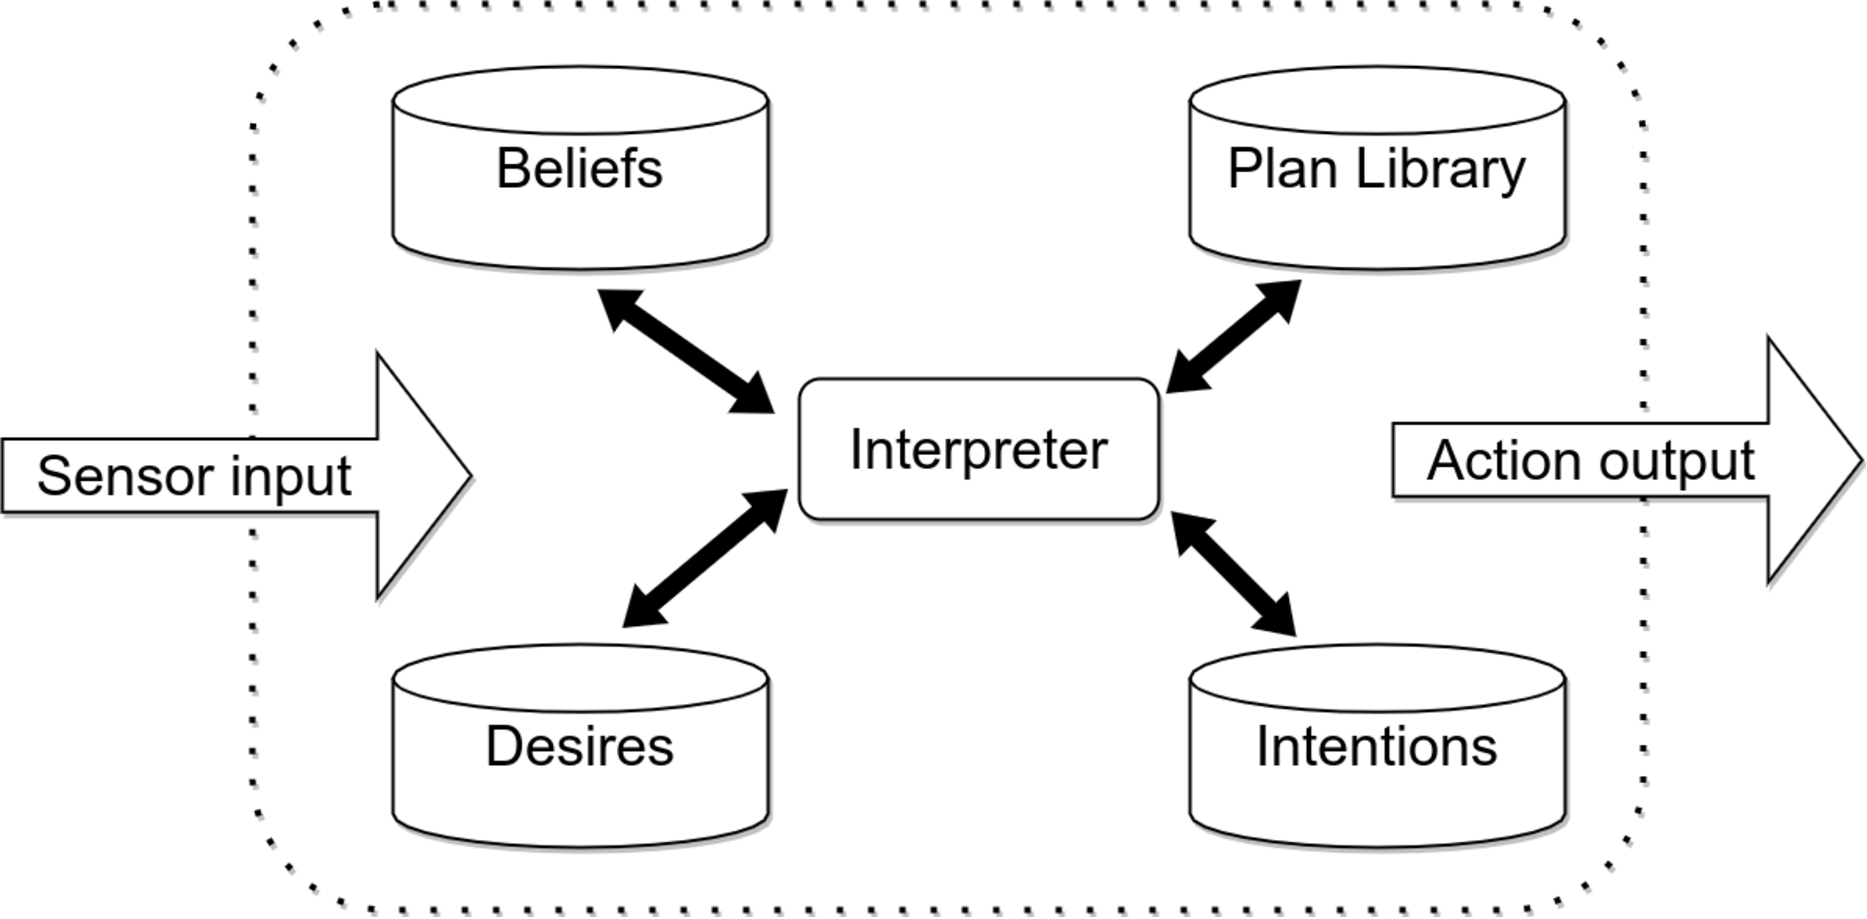
\includegraphics[scale=0.18]{BDI.pdf}
 % bdi1.pdf: 0x0 px, 300dpi, 0.00x0.00 cm, bb=
 \caption{{\tiny Adapted from \cite{bordini2007}}}
\end{figure}
\end{columns}

\vspace{.3cm}
\scriptsize
\underline{Agent-oriented programming}: languages and interpreters implement items \textcolor{blue}{1} to \textcolor{blue}{9} above. The programmer focuses on item \textcolor{blue}{10}.

\end{frame}

\begin{frame}{The Jason Language}

\begin{columns}
 \column{.7\textwidth}
 A language for programming BDI agents\\ 
 \link{https://jason-lang.github.io}{https://jason-lang.github.io}\\
 {\tiny  In this course, \textit{Jason} is used with the \link{https://jacamo-lang.github.io/}{JaCaMo framework} \cite{boissier2020}}
 \column{.3\textwidth}
  \begin{figure}[htbp]
 \centering
 
\includegraphics[scale=.2]{JasonBook.png}
 % jason_bdi.png: 523x386 px, 72dpi, 18.45x13.62 cm, bb=0 0 523 386
\end{figure}
\end{columns}

\vspace{.5cm}

{\bf Agent Programming} with high-level BDI constructs\\
\vspace{-.2cm}{\tiny in Jason, we program beliefs, desires, and intentions}\\
{\tiny instead of programming variables, functions, procedures, methods, objects, ...}

\vspace{.5cm}
{\bf Agent Execution} in the form of a reasoning cycle\\
\vspace{-.2cm}{\tiny a Jason agent remains in continuous execution, observing the world, updating its beliefs}\\
\vspace{-.2cm}{\tiny evaluating the desires that can be satisfied, selecting plans to execute them,}\\
{\tiny putting the plans into execution, and restarting the cycle}
\end{frame}

\begin{frame}{The Jason Language}
 
\begin{figure}[htbp]
\centering
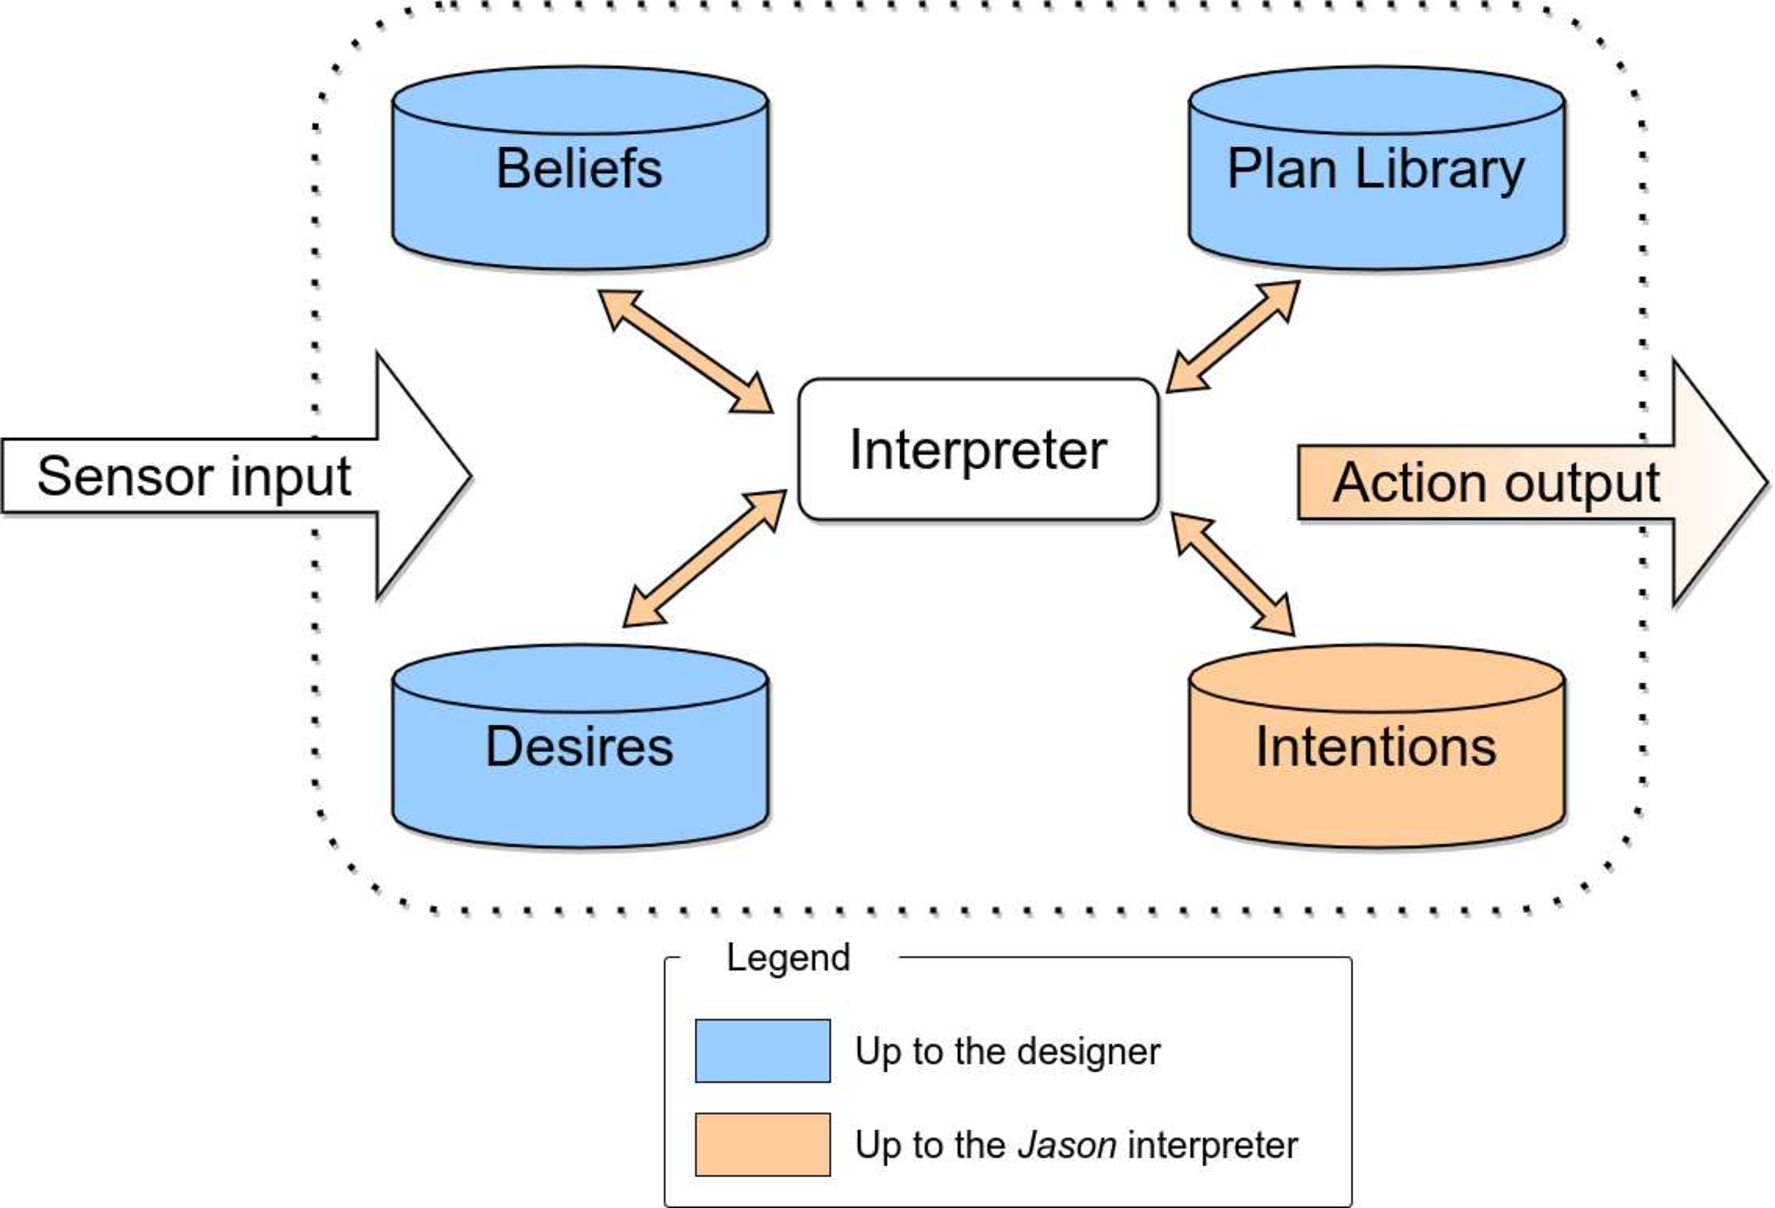
\includegraphics[scale=.3]{BDI_colors.pdf}
 % jason_bdi.png: 523x386 px, 72dpi, 18.45x13.62 cm, bb=0 0 523 386
\end{figure}

\end{frame}


\begin{frame}{Agent Oriented Programming with \textit{Jason}{\tiny \cite{bordini2007} }}

\footnotesize

 MAS development platform based on an extended version of AgentSpeak {\tiny \cite{rao1996}}\\\vspace{.3cm}
 
 Agents are implemented with high level constructs of the BDI model {\tiny \cite{bratman1988}}\\ \vspace{.3cm}
 
 In this course, \textit{Jason} is used with the JaCaMo framework {\tiny \cite{boissier2020}}
 
\end{frame}


\begin{frame}{Agents}
   \begin{figure}[htbp]
    \centering
        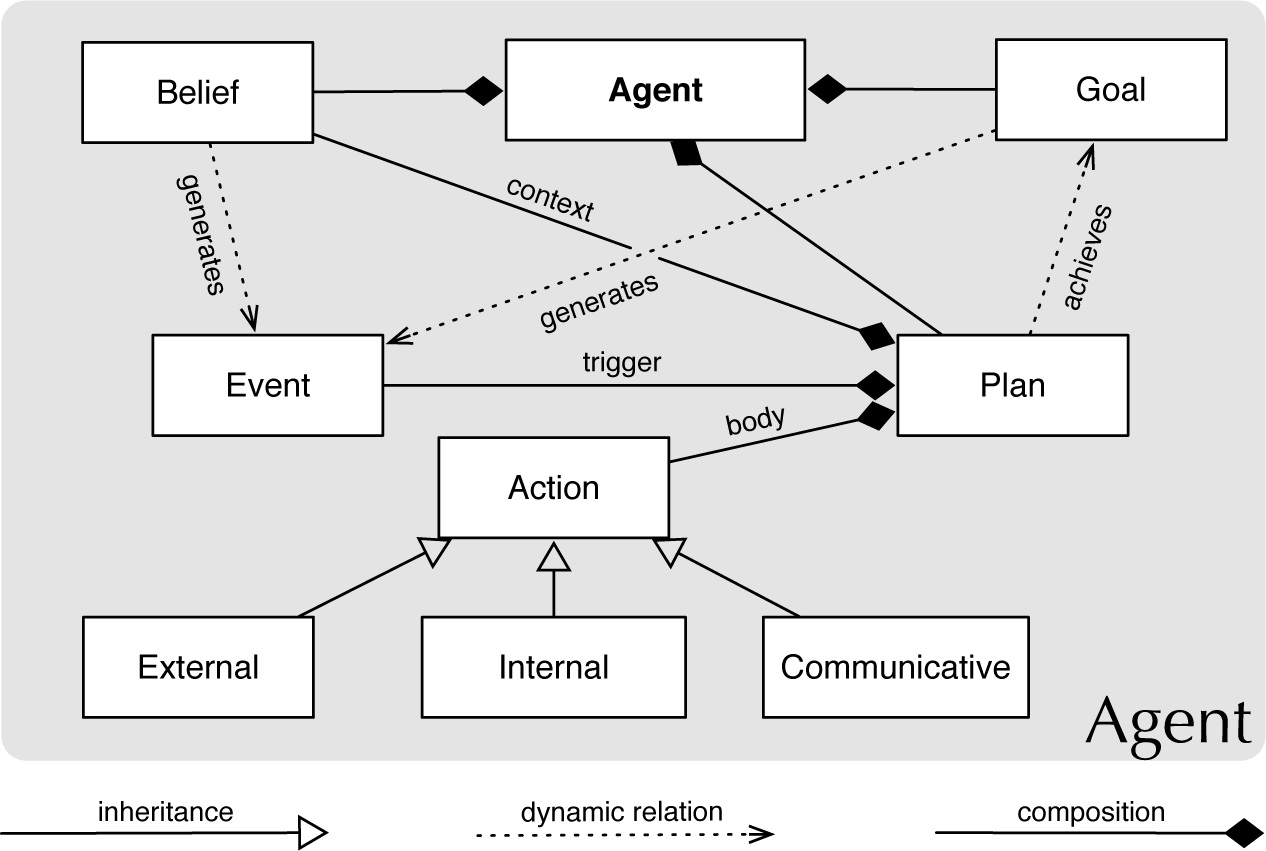
\includegraphics[scale=.2]{agent-jacamo-book-2.png}
        \caption{
        \fontsize{7pt}{2pt}\selectfont
            \cite{boissier2020}
        } 
\end{figure}


\end{frame}

\begin{frame}{Agents}
\framesubtitle{{\scriptsize Essential Jason constructs}}

   \begin{columns}
     \column{.48\textwidth} \footnotesize
         {\bf Beliefs: } information available to the agent
         {\tiny about the environment, other agents, itself...}\\
         \vspace{.5cm}
        {\bf Goals: }states of affairs the agent wants to bring about\\
        \vspace{.5cm}
        {\bf Plans: }recipes for action (agent's know how)
     \column{.48\textwidth}
        \begin{figure}[htbp]
            \centering
            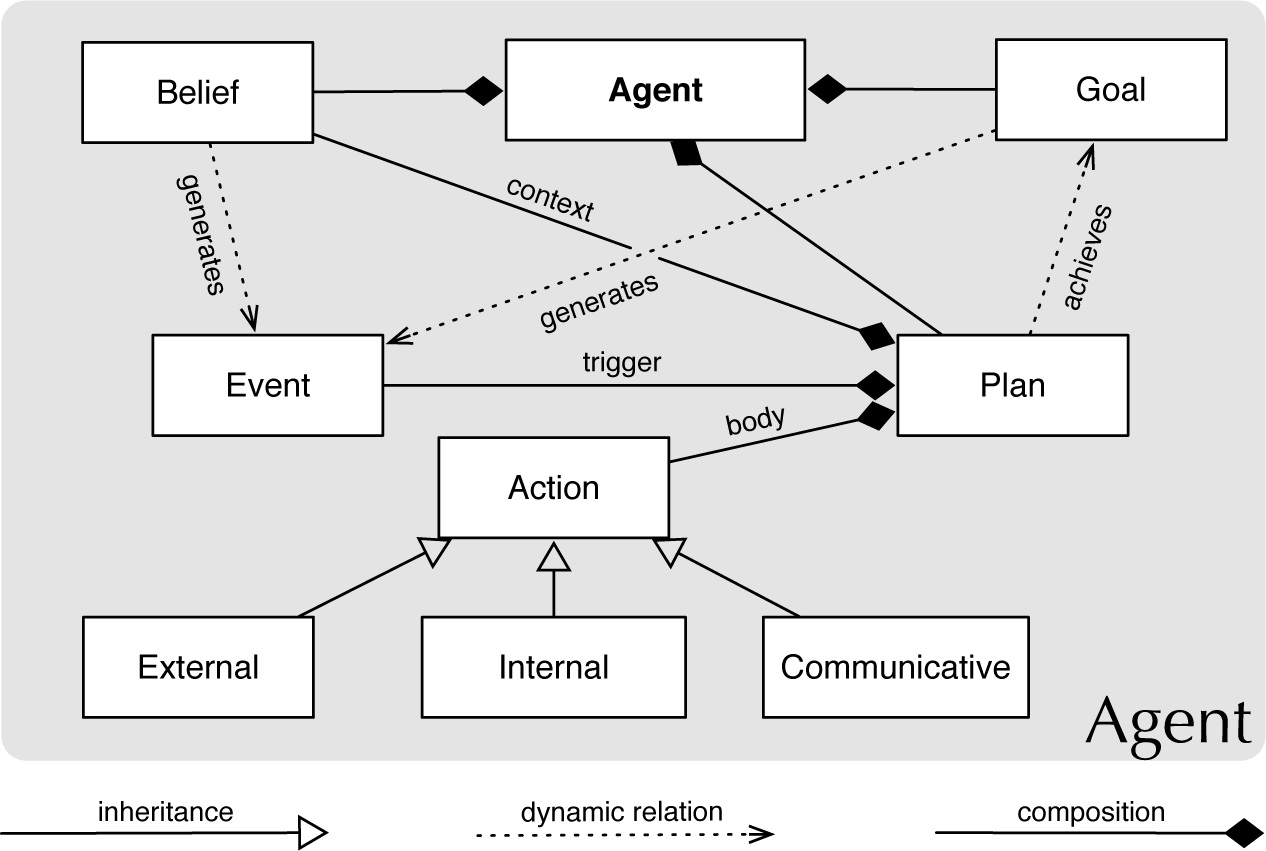
\includegraphics[scale=.12]{agent-jacamo-book-2.png}
            \caption{{\tiny \cite{boissier2020}}}
        \end{figure}
        
   \end{columns}

\end{frame}


\begin{frame}[fragile]{Hello World - The first \jacamo program}

\begin{alltt}
   
   \belief{language(english).} \comment{initial belief}
   \desire{!greet.} \comment{//initial desire (or \textit{goal})}
   
   \comment{//plans to satisfy the goal \textit{greet}} 
   \planhead{+!greet} : \belief{language(english)}
       <- \instruction{.print("hello world.")}.
    
   \planhead{+!greet} : \belief{language(french)} 
       <- \instruction{.print("bonjour.")}.    
\end{alltt}
\end{frame}

\begin{frame}{Hello World - The first \jacamo application - version 1}
%
%
 \begin{columns}
   

   \column{.5\textwidth}
     \begin{block}{\jacamo app specification}
     \begin{alltt}\scriptsize
        mas agents\_intro \{\\
        \ \ agent bob: personal\_assistant.asl
      \}      
      \ \\
      \ \\
      \ \\
      \ \\
      \ \\
      \ \\
      \ \\
     \end{alltt}
     \end{block}

     \column{.5\textwidth}
     \begin{block}{agent specification}
      \scriptsize
      \begin{alltt}
         \belief{language(english).} \comment{initial belief}\\
         \desire{!greet.} \comment{//initial desire (or \textit{goal})}\\
         %\vspace{0.8cm} 

         \comment{//plans to satisfy the goal}  \\
         \planhead{+!greet} : \belief{language(english)} \\
         \ \ \ \ <- \instruction{.print("hello world.")}.\\
    
         \planhead{+!greet} : \belief{language(french)} \\
         \ \ \ \ <- \instruction{.print("bonjour.")}.    
      \end{alltt}
     \end{block}
     
 \end{columns}

\end{frame}


\begin{frame}{Hello World - The first \jacamo application - version 2}
%
%
 \begin{columns}
   

   \column{.5\textwidth}
     \begin{block}{\jacamo app specification}
     \begin{alltt}\scriptsize
        mas agents\_intro \{\\
        \ \ agent bob: personal\_assistant.asl\{\\
        \ \ \ \ goals: \desire{greet}\\
        \ \ \ \ beliefs: \belief{language(english)}\\
        \ \ \} \\   
      \}      
      \ \\
     \end{alltt}
     \end{block}

     \column{.5\textwidth}
     \begin{block}{agent specification}
      \scriptsize
      \begin{alltt}
         
         \comment{//plans to satisfy the goal}  \\
         \planhead{+!greet} : \belief{language(english)} \\
         \ \ \ \ <- \instruction{.print("hello world.")}.\\
    
         \planhead{+!greet} : \belief{language(french)} \\
         \ \ \ \ <- \instruction{.print("bonjour.")}.    
      \end{alltt}
     \end{block}
     
 \end{columns}

\end{frame}


\begin{frame}{Hello World - The first \jacamo program}
%
%
   

\begin{figure}[htbp]
 \centering
 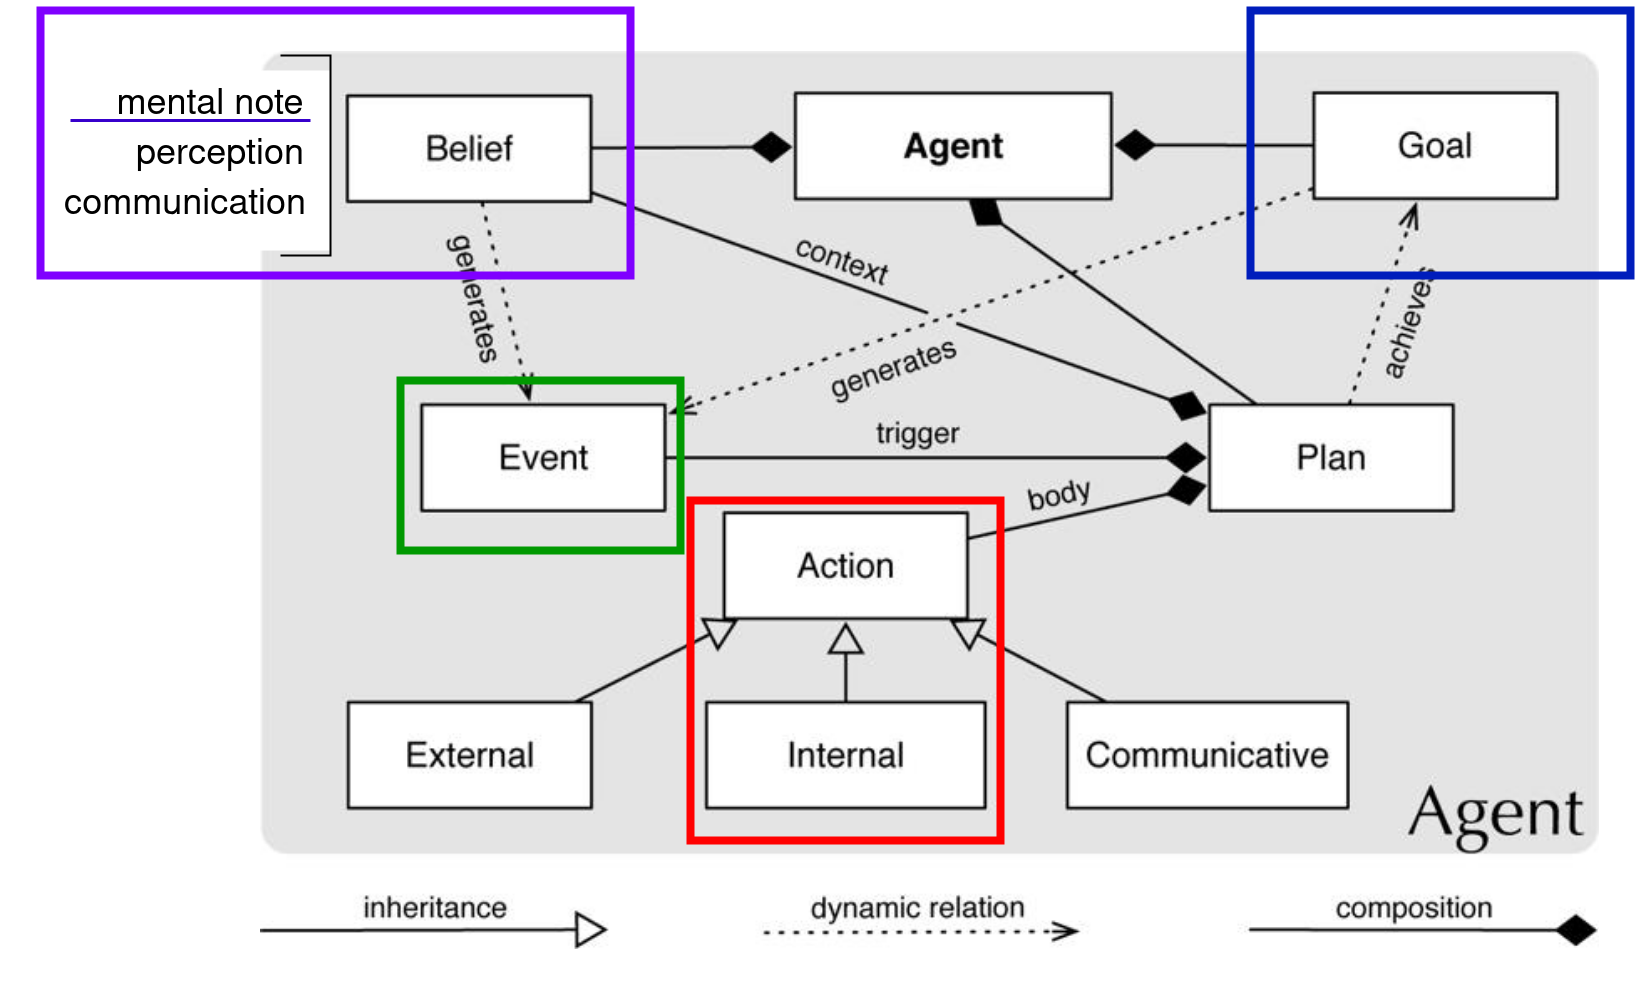
\includegraphics[scale=.12]{agent-jacamo-book-maiquel-abstractions-1.drawio.png}
  \vskip -1.0em % Adjust the value here as needed to change the distance
 \caption{{\tiny adapted from \cite{boissier2020}}}
\end{figure}

\ssmall
 \vspace{-.5cm}
 \begin{columns}
   

   \column{.5\textwidth}
   {\setbeamerfont{block title}{size=\ssmall}
     \begin{block}{\jacamo app specification}
     \begin{alltt}
        mas agents\_intro \{\\
        \ \ agent bob: personal\_assistant.asl\{\\
        \ \ \ \ goals: \desire{greet}\\
        \ \ \ \ beliefs: \belief{language(english)}\\
        \ \ \} \\   
      \}      
      \ \\
      \ \\
      \ \\
     \end{alltt}
     \end{block}}

     \column{.5\textwidth}
     {\setbeamerfont{block title}{size=\ssmall}
     \begin{block}{agent specification}
      \begin{alltt}
         \desire{!greet.} \comment{//initial desire (or \textit{goal})}\\
         %\vspace{0.8cm} 

         \comment{//plans to satisfy the goal}  \\
         \planhead{+!greet} : \belief{language(english)} \\
         \ \ \ \ <- \instruction{.print("hello world.")}.\\
    
         \planhead{+!greet} : \belief{language(french)} \\
         \ \ \ \ <- \instruction{.print("bonjour.")}.    
      \end{alltt}
     \end{block}
     }
 \end{columns}

 \vfill
 {\tiny Go to exercises 2.1.1 to 2.3.3}
\end{frame}




\begin{frame}{Main agent constructs -- Beliefs}
 
 \begin{block}{Syntax}
  Beliefs are represented by annotated literals of first order logic \\
  \belief{$functor(term_1,\cdots,term_n)[annot_1,\cdots,annot_n]$}
 \end{block}
 
 \begin{block}{Example} \footnotesize
  \begin{alltt}
     \belief{language(english)[source(self)]} \comment{//added by the agent itself}\\
     \belief{temperature(20)[source(percept)]} \comment{//added by perception}\\
     \belief{friend(bob,alice)[source(bob)]} \comment{//added by communication from bob}
  \end{alltt}

     
 \end{block}

 
\end{frame}

\subsection{Beliefs}

\begin{frame}[fragile]{Where do the beliefs come from? I}


\begin{block} {Coded as agent's initial beliefs {\tiny either in the .asl or in the .jcm file}}

 
 
  \begin{alltt}\tiny
   \belief{language(english).} \comment{//initial belief}
   \desire{!greet.} \comment{//initial goal}

   \comment{//plan to satisfy the goal}  
   \planhead{+!greet} : \belief{language(english)} 
       <- \instruction{print(``Hello world'')}.
    

\end{alltt}
\end{block}

\begin{block}{Added as part of plans}
  \begin{alltt}\tiny
   \belief{language(english).} \comment{//initial belief} 
   \desire{!greet.} \comment{//initial goal}

   \comment{//plan to satisfy the desire}  
   \planhead{+!greet} : \belief{language(english)}
        <- \instruction{print(``Hello world'')}.
           \belief{-last\_greeting\_date(friday);} \comment{//remove belief}
           \belief{+last\_greeting\_date(saturday);} \comment{//add belief}
           \belief{-+last\_greeting\_date(sunday).} \comment{//update belief}

\end{alltt}
\end{block}

%Beliefs added by the agent itself include the \texttt{source(self)} annotation\\
%e.g.: \texttt{\belief{language(english)[source(self)]}}

 
\end{frame}




\begin{frame}{Where do the beliefs come from? II}
%
 
 {\bf Beliefs added by communication}
 \vspace{.5cm}
 \begin{itemize}
  \item Have the \texttt{source(ag) annotation}\\
  {\tiny where ag is the agent that provides the information}
  \item Dynamics: 
   
   \begin{itemize}\footnotesize
     \item when the agent receives a \textit{tell} message, its content becomes a new belief\\
     \begin{alltt}
       \instruction{.send(tom,tell,lier(alice));}\comment{//sent by bob}\\      
       \comment{//adds lier(alice)[source(bob)] in tom's bb}
     \end{alltt}
     
     \vspace{.8em}
     
     \item when the agent receives an \textit{untell} message, the corresponding belief is removed from the receiver's belief base\\
     \begin{alltt}
       \instruction{.send(tom,untell,lier(alice));}\comment{//sent by bob}\\
        \comment{//removes lier(alice)[source(bob)] in tom's bb}
     \end{alltt}
    \end{itemize} 
  \end{itemize}
 \vfill
 {\tiny Go to exercise 2.3.4}
\end{frame}

\begin{frame}[fragile]{Where do the beliefs come from? III}

   
   From the agent's perception of the environment\\ 
   
   %\vspace{.3cm}
   
   \scriptsize
   include the annotation \texttt{source(percept)}\\
   are automatically updated as perceptions change\\
   
   %\vspace{1cm}
   \begin{alltt}\scriptsize
     \belief{language(english).}
     
     \desire{!greet.}

     \planhead{+!greet} : \belief{language(english)} 
               \belief{temperature(X)[source(percept)]} \& X <= 10 
        <- \instruction{.print("hello world.");}
           \instruction{.print("It is so cool").}
 
   \end{alltt}

   %{\tiny \link{http://maiquelb.github.io/sepex2020/codes/greet_beliefs_env.zip}{download}} 
   
   \vfill
   
   {\tiny Go to Exercise 2.3.5}
 
\end{frame}


\begin{frame}{Main agent constructs -- Goals}

\footnotesize
 
 \vspace{0.5cm}
 
 {\bf Goals} correspond to the notion of \textit{desire} from BDI.\\ \vspace{.3cm}
 
 Represent the states of the world the agent wants to bring about\\
 \vspace{0.5cm}
 
 \begin{block}{Syntax}
  $!<goal\_identifier>\mathtt{(<argument_1,\cdots,argument_n>)}$\\
  {\tiny (arguments are optional)}
 \end{block}

 \vspace{0.5cm}
 
 Types of goals:
   \begin{itemize}
   \item declarative goals: goals about states {\tiny (e.g.~\texttt{!be\_at(wesaac)})}
   \item procedural goals: goals about (sequence of) actions {\tiny (e.g.~\texttt{!go\_to(wesaac)})}
  \end{itemize}
 
% Types of goals:
% \begin{itemize}
%  \item \textit{achievement goal}: goal to do\\
%  \ \ \ \ \ \ \ \ \ \ \ \ \ \ \ \ \ \ \ \ \ \ \ \ \ {\scriptsize syntax: \texttt{!g.} : the agent wants to achieve \textit{g}}
%  \begin{itemize}
%   \item declarative goal: goal about a state
%   \item procedural goal: goal about a (sequence of) action
%  \end{itemize}

%  \item \textit{test goal}: objetivo de saber\\
%  \ \ \ \ \ \ \ \ \ \ \ \ \ \ \ \ \ \ \ \ \ \ \ \ \ {\scriptsize sintaxe: \texttt{?g.} : the agent wants to know \textit{g}}
% \end{itemize}

%\begin{block}{Exemplos}
% \desire{!greet.} \comment{//achievement goal}\\ \vspace{.2cm}
% \desire{?is\_holiday. \comment{//test goal}}
%\end{block}


\vfill
 \scalebox{0.8}{\tiny Declarative and procedural goals are \textit{achievement goals}, which are goals to do.}\\ \scalebox{0.8}{\tiny Jason considers also \textit{test goals}, which are goals to know. Test goals are not the focus in this presentation.}
 
\end{frame}





\begin{frame}[fragile]{Where do the goals come from? I }
 

\begin{block}{Agent's initial goal {\tiny either in the .asl or in the .jcm file}}
 \begin{alltt}\tiny
   \belief{language(english).} \comment{//belief} 
   \desire{!greet.} \comment{//initial goal}

   \comment{//plan to satisfy the goal}  
   \planhead{+!greet} : \belief{language(english)}
       <- \instruction{print("Hello world")}.
    

\end{alltt}

\end{block}

%\vspace{1cm}

 
\begin{block}{Part of plans}
\begin{alltt}\tiny
   \belief{language(english).} \comment{//belief} 
   \desire{!greet.} \comment{//initial goal}
   
   \comment{//plan to satisfy the desire}  
   \planhead{+!greet} : \belief{language(english)}
       <- \instruction{print("Hello world.")};
          \comment{//add test [sub]goal}
          \desire{?raining(now);} 
          \comment{//add achievement [sub]goal}
          \desire{!check\_temperature.} 
\end{alltt}
\end{block}


\end{frame}



\begin{frame}{Where do the goals come from? II}

   
    {\bf Goals added by communication}
    
   
   \begin{itemize}\footnotesize
     \item when the agent receives an \textit{achieve} message, its content becomes an achievement goal {\tiny annotated with the sender of the message}\\
     \begin{alltt}
       \instruction{.send(tom,achieve,write(book));}\comment{//sent by bob}\\      
       \comment{//adds new goal write(book)[source(bob)] for Tom}
     \end{alltt}
     
     \item when the agent receives an \textit{unachieve} message, the goal corresponding to the message's content is removed
     \begin{alltt}
       \instruction{.send(tom,unachieve,write(book));}\comment{//sent by bob}\\      
       \comment{//removes the goal write(book)[source(bob)] for Tom}
     \end{alltt}
    
  

    \item when the agent receives an \textit{askOne} or \textit{askAll} message, the content is a new test goal  {\tiny annotated with the sender of the message}\\
    \begin{alltt}
       \instruction{.send(tom,askOne,published(P),Answer);}\comment{//sent by bob}\\      
       \comment{//adds new goal ?published(P)[source(bob)] for Tom}\\
       \comment{//the response of Tom unifies with Answer}
     \end{alltt}
    \end{itemize} 
\end{frame}





\subsection{Plans}


\begin{frame}{Plans}
 
 %\begin{center}
    
%\end{center}
    \begin{columns}
        \column{.7\textwidth}
        \texttt{triggering\_event : \belief{context} \textless -- \instruction{body}.}\\ \vspace{1cm}
        
        \scriptsize
        \texttt{triggering\_event}: event the plan is meant to handle\\\vspace{.2cm}
        \texttt{context}: circumstances in which the plan is selected\\ \vspace{.2cm}
        \texttt{body}: course of action to be followed when the plan is\\
        \ \ \ \ \ \ \ \ \ selected\\
            
        \column{.3\textwidth} \tiny
            \begin{block}{Triggering events}
            \texttt{+b} (belief addition)\\
            \texttt{-b} (belief deletion)\\
            
            \texttt{+!g} (achievement goal addition)\\
            \texttt{-!g} (achievement goal deletion)\\
            
            \texttt{+?g} (test goal addition)\\
            \texttt{-?g} (test goal deletion)\\
             
            \end{block}

    \end{columns}


 
\end{frame}



\begin{frame}{Plans \textminus\ context}

\footnotesize
Context is typically formed of 
conjunctions of beliefs that the agent is required to
have at the time of choosing the plan

\centering
\begin{alltt}\scriptsize
 \ \ \ \ \ \ \planhead{+!greet} : \belief{language(english)} \& \belief{temperature(X)} \& X>=30\\
    \ \ \ \ \ \ \ \ \ <- .\ .\ .\\
\end{alltt}


\begin{columns}
 \column{.4\textwidth}
   \begin{block}{Boolean operators}
   \scriptsize
   \begin{center}
     \begin{tabular}{cl}
        \texttt{\&} & (and)\\
        \texttt{$\mid$} & (or)\\
        \texttt{not} & (not)\\
        \texttt{$=$} & (not)\\
        \texttt{$>$,$>=$,$<$,$<=$} & (relational)\\
        \texttt{==} & (equals)\\
        \texttt{$\setminus ==$} & (different)\\
        \\
     \end{tabular}
   \end{center}

   \end{block}
 \column{.4\textwidth}
   \begin{block}{Arithmetic operators}
    \footnotesize
    \begin{center} 
     \begin{tabular}{cl}
        \texttt{+} & (sum)\\
        \texttwelveudash & (subtraction)\\    
        \texttt{$*$} & (multiply)\\
        \texttt{/} & (divide)\\
        \texttt{{\bf div}} & divide -- integer\\
        \texttt{{\bf mod}} & remainder\\
        \texttt{$**$} & power\\
        %\texttt{$=$} & (not)\\
        %\texttt{$>$,$>=$,$<$,$<=$} & (relational)\\
        %\texttt{==} & (equals)\\
        %\texttt{$\setminus ==$} & (different)\\
     \end{tabular}
    \end{center}
   \end{block}

\end{columns}


 
\end{frame}



\begin{frame}[fragile]{Plans - body} 
 
What may the plan body include?
 
 \begin{alltt}\scriptsize
    \planhead{+rain} : \belief{time\_to\_leave(T)} \& clock.now(H) \& \belief{H>=T}
       <- \desire{!g1}; \comment{//new subgoal}
          \desire{!!g2}; \comment{//new goal}
          \desire{?b(X)}; \comment{//new test goal}
          \belief{+b1(T-H)}; \comment{//add mental note}
          \belief{-b2(T+H)}; \comment{//remove mental note}
          \belief{-+b3(T*H)}; \comment{//update mental note}
          \instruction{close(door)}; \comment{//external action}
          \instruction{.print(``Go!'')}. \comment{internal action}
 \end{alltt}

 
 
\end{frame}

\subsubsection{Plans and actions}
\begin{frame}{Plans \textit{vs}. actions of agents}

\footnotesize

Plans may include {\bf actions} the agents are expected to execute.\\ \vspace{1cm}

But...\\
Where are these actions implemented? \vspace{1cm}

There are two kinds of actions:
\begin{itemize}
 \item Internal actions
 \item External actions
\end{itemize}
 
\end{frame}

\begin{frame}{External actions}
 
 Executed on elements external to the agent's implementation
 {\tiny i.e. \textit{environment}}\\ 
 %\vspace{.5cm}
 %Provocam efeitos sobre o \textit{ambiente}.\\
 
 \vspace{.5cm}
 
 In \jacamo, the environment is based on \textsf{CArtAgO} {\tiny (details \link{http://cartago.sourceforge.net/}{here} and \link{https://raw.githubusercontent.com/CArtAgO-lang/cartago/master/docs/cartago_by_examples/cartago_by_examples.pdf}{here})}
 

\end{frame}
 
 

\begin{frame}{Internal actions}

\footnotesize

 
\begin{itemize}
 \item are not necessarily performed upon an external device
 \item are part of the agent implementation
 \item are executed as part of the agent reasoning cycle
 \item are available to the agent in any environment
\end{itemize}

%\vspace{.5cm}

\begin{columns}
 \column{.7\textwidth}
 \textit{Internal actions} are implemented in Java
\begin{itemize}\scriptsize
 \item {\scriptsize New \textit{internal actions} can be implemented}\\ {\tiny and added to the agent}
 %\item O nome da ação é precedido por ``\texttt{.}''\\ {\tiny ex. \texttt{.print(``Hello'')}} 
 \item Jason provides a default set of internal actions\\
 {\tiny available to every Jason agent} 
 \item More info \link{http://jason.sourceforge.net/api/jason/stdlib/package-summary.html}{here}
\end{itemize}

\column{.3\textwidth}
\begin{block}{{\scriptsize Example} {\tiny (download \link{http://maiquelb.github.io/sepex2020/codes/example_internal_actions.zip}{here})}}% {\tiny download \link{http://maiquelb.github.io/sepex2020/codes/example_internal_actions.zip}{aqui}}}
\begin{alltt}\tiny
\planhead{+!start} <- \\
   \ \ \ .print("hello world.");\\
   \ \ \ .random(R); .print(R);\\
   \ \ \ .date(Y,M,D); \\ \ \ \ .print(Y,"-",M,"-",D);\\
   \ \ \ .time(H,MN,S); \\ \ \ \ .print(H,"-",MN,"-",S).\\
   \ \\ \ \\ \ \\ \ \\ \ \\ \ \\
\end{alltt}
\end{block}

\end{columns}





\end{frame}




\section{Introduction to Jason-ROS}

\begin{frame}
 

 \HUGE
\centering
Part III\\
Introducton to \\
Jason-ROS 
 
\end{frame}


\begin{frame}{Autonomous robots with BDI agents and ROS}

\footnotesize
{\bf Assumptions:}
\vspace{.3cm}

\begin{itemize}\scriptsize
 
 
 \item BDI agents are a suitable approach for developing systems\\
 with features such as  proactivity, autonomy, deliberative skills,\\ and social abilities
 
 \vspace{.3cm}
 
 \item ROS is a suitable tool for robot programming \\
 {\tiny but does not provide features such as proactivity, autonomy, deliberative skills, and social abilities}
 
 \vspace{.3cm}
 
 \item Conciliating BDI agent programming with ROS to have robots with these features
 \begin{itemize} \ssmall
  \item integrate the BDI model with the ROS programming model  
  \item integrate AOP tools with the ROS platform
 \end{itemize}

\end{itemize}

 
\end{frame}


\begin{frame}{Autonomous robots with Jason and ROS}

{\bf Assumptions:}\vspace{.5cm}

Jason is suitable for BDI agent programming\\
{\tiny the behaviour of a robot may be fully specified in Jason}\\ \vspace{.5cm}

Programming Jason-ROS robots requires to connect
\begin{itemize}
 \item  perceptions of the agent with the robot sensors \\
 {\tiny whose values are recorded in ROS topics}
 \item actions of the agent with the physical effectors\\
 {\tiny controlled by both ROS topics and actions}
\end{itemize}
\end{frame}


\begin{frame}{Jason-ROS}

 Jason-ROS extends the default Jason agents: \vspace{.5cm}
 \begin{itemize}
  \item perceptions may be obtained from physical sensors\\ {\tiny whose values are recorded in ROS topics} \vspace{.2cm}
  
  \item actions may be realized by physical actuators\\
       {\tiny controlled by ROS topics and services}
 \end{itemize}

 
\vfill
{\tiny Jason-ROS is availale \link{https://github.com/embedded-mas/jason-ros}{here}}.\\
{\tiny It is part of a more comprehensive work to combine Jason agents with physical devices available \link{https://github.com/embedded-mas/embedded-mas/}{here}}.
 
\end{frame}

\begin{frame}{Jason-ROS}
 \centering
 
 \begin{figure}
 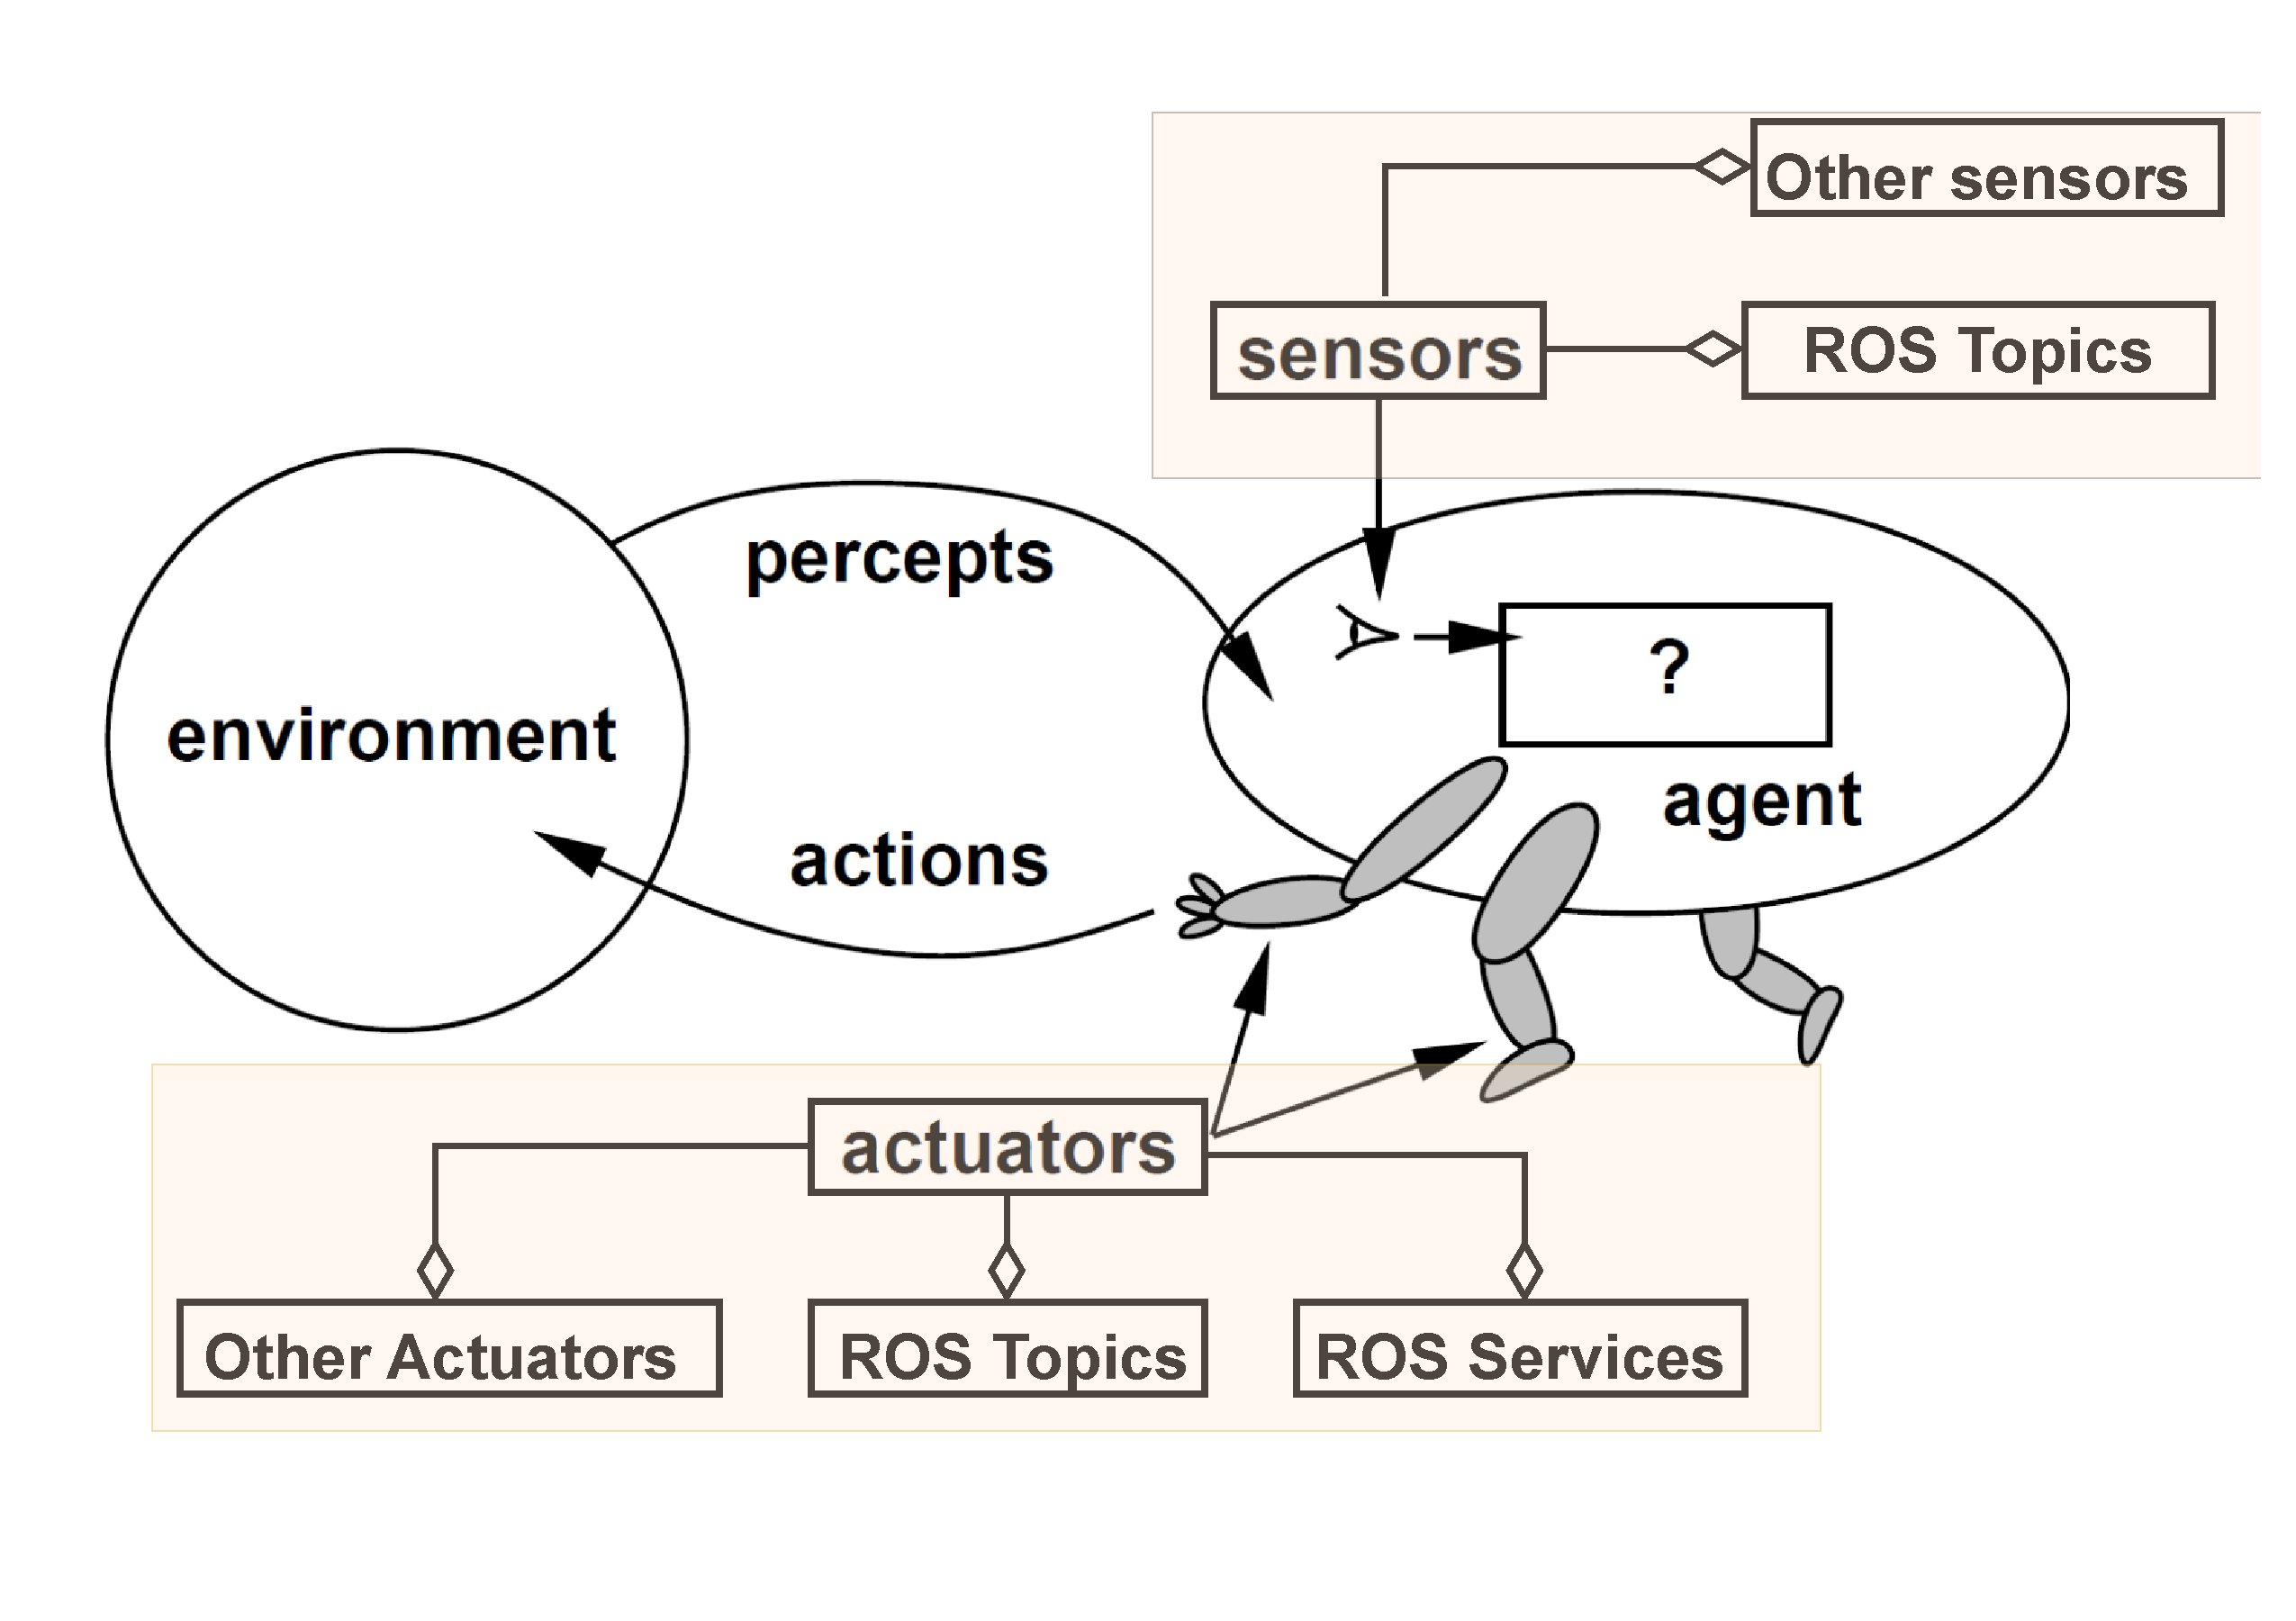
\includegraphics[scale=.18]{jason-ros-agent-russel-norvig.pdf}
  \caption{{\tiny Image adapted from~\cite{russel1995}}}
 \end{figure}
 
 \end{frame}


\begin{frame}{Jason-ROS}

\begin{figure}
 \centering
 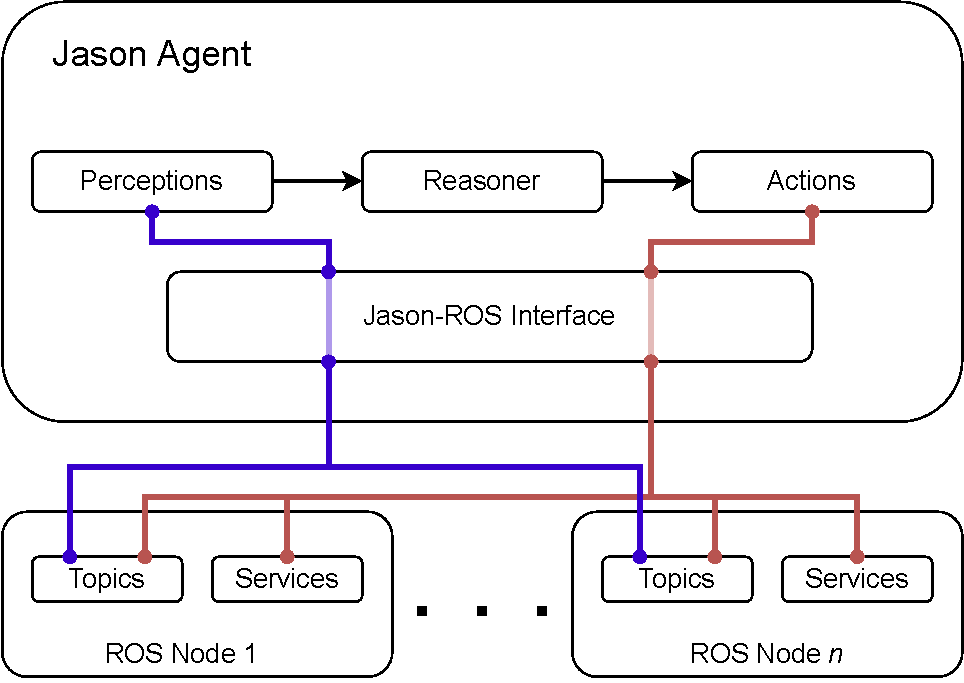
\includegraphics[scale=.5]{Jason-ROS.pdf}
 % Jason-ROS.pdf: 0x0 px, 300dpi, 0.00x0.00 cm, bb=
\end{figure}

\end{frame}

\begin{frame}{Jason-ROS}

\begin{figure}
 \centering
 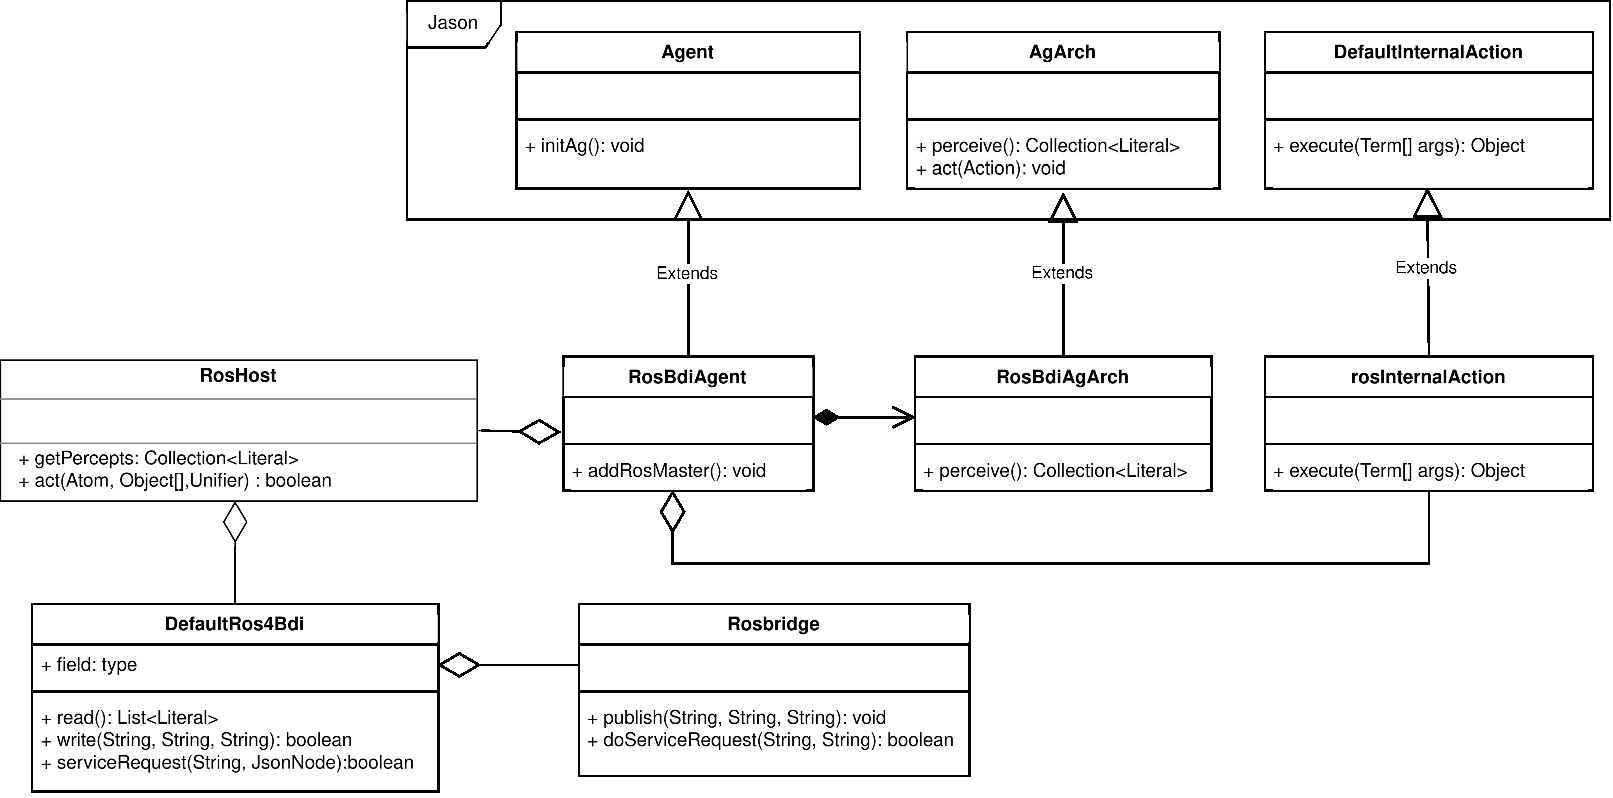
\includegraphics[scale=.4]{uml_jason_ros.drawio.pdf}
 % Jason-ROS.pdf: 0x0 px, 300dpi, 0.00x0.00 cm, bb=
\end{figure}
 
\end{frame}

\begin{frame}[fragile]{Jason-ROS}

\scriptsize
\begin{block}{Set up of a Jason-ROS agent in JaCaMo}
  \begin{alltt}\scriptsize
   mas jason\_ros \{  
   \ \ \ agent robot1: ros\_agent.asl \{
   \ \ \ \ \ \ \colorbox{yellow}{ag-class}: \colorbox{cyan}{embedded.mas.bridges.jacamo.ros.RosBdiAgent}
   \ \ \ \ \ \ ag-arch: embedded.mas.bridges.jacamo.ros.RosBdiAgArch
   \ \ \ \}
  \}
  \end{alltt}    
\end{block}

\footnotesize
\colorbox{yellow}{{\bf ag-class}}: defines the Java class that implements the essential functions\\ \ \ \ \ \ \ \ \ \ \ \ \ \ and data structures for running an agent\\

\vspace{.3cm}

\colorbox{cyan}{{\bf RosBdiAgent}}: 
\begin{itemize}
 \item extends the \href{https://github.com/jason-lang/jason/blob/main/jason-interpreter/src/main/java/jason/asSemantics/Agent.java}{\underline{\textcolor{blue}{default Agent class of Jason}}}\\
 \item provides means for 
 \begin{itemize}\scriptsize
   \item including topics among the perception sources of the agent
   \item linking the action repertory to service calls and topic writings
   %\item get percepts from topics
   %\item realize actions by writing in topics and requesting services
 \end{itemize}
 
\end{itemize}


 
\end{frame}


\begin{frame}[fragile]{Jason-ROS}

\scriptsize
\begin{block}{Set up of a Jason-ROS agent in JaCaMo}
  \begin{alltt}\scriptsize
   mas jason\_ros \{  
   \ \ \ agent robot1: ros\_agent.asl \{
   \ \ \ \ \ \ ag-class: embedded.mas.bridges.jacamo.ros.RosBdiAgent
   \ \ \ \ \ \ \colorbox{yellow}{ag-arch}: \colorbox{cyan}{embedded.mas.bridges.jacamo.ros.RosBdiAgArch}
   \ \ \ \}
  \}
  \end{alltt}    
\end{block}

\footnotesize
\colorbox{yellow}{\bf ag-arch}: defines the Java class that implements the essential functions\\ \ \ \ \ \ \ \ \ \ \ \ \ \ and data structures for the agent to interact with the external world\\ \ \ \ \ \ \ \ \ \ \ \ \ \  {\tiny in the perceive and act phases of the reasoning cycle}

\vspace{.3cm}

\colorbox{cyan}{\bf RosBdiAgArch}: 
\begin{itemize}
 \item extends the \href{https://github.com/jason-lang/jason/blob/main/jason-interpreter/src/main/java/jason/architecture/AgArch.java}{\underline{\textcolor{blue}{default agent architecture of Jason}}}\\
 \item includes the reading of topics in the perceiving process
\end{itemize}


 
\end{frame}





\begin{frame}{Programming Jason-ROS Robots}{Connecting the agents' abstractions to ROS resources}

The cognitive portion of the agent is programmed in .asl files\\ \vspace{.5cm}
 
The connection between cognitive and physical portion (controlled by ROS)
is specified in a .yaml configuration file\\ \vspace{-.2cm}
{\tiny each agent has its own .yaml file}\\ \vspace{-.2cm}
{\tiny the .yaml file has the same name as the agent name (which may differ from the .asl file name)}\\ \vspace{-.2cm}
{\tiny the same .asl may lead to agents with different conenctions Jason-ROS}

 
\end{frame}



\begin{frame}[fragile]{Programming Jason-ROS Robots}{Connecting the agents' abstractions to ROS resources}

    \footnotesize
    
    A Jason-ROS agent is composed of a set of \textit{devices}\\
    
    A \textit{device} is a physical portion of the agent,\\ composed of a set of sensors and actuators {\tiny (\tiny controled by ROS, in this case)}
    
    \vspace{.5cm}
    
  \begin{columns}
  \column{.33\textwidth}
  \column{.33\textwidth}
            \begin{block}{{\ssmall Jason-ROS configuration file}}
                \scriptsize
                \begin{alltt} \tiny
- \colorbox{yellow}{\yamlkey{device\_id}: \yamlvalue{device_1}}
    ...
- \colorbox{yellow}{\yamlkey{device\_id}: \yamlvalue{device_2}}      
    ...
- \colorbox{yellow}{\yamlkey{device\_id}: \yamlvalue{device_n}}    
                \end{alltt}

            \end{block}    
  \column{.33\textwidth}            
 \end{columns}
\end{frame}


\begin{frame}[fragile]{Programming Jason-ROS Robots}{Connecting the agents' abstractions to ROS resources}

    \footnotesize
    \texttt{{\bf device\_id}}: identifies a connection with an external portion of the agent\\ 
    
    \vspace{-.5cm}
    
    \ \ \ \ \ \ \ \ \ \ \ \ \ \ {\tiny that, in this case, is a ROS host}

    
    \begin{columns}
       \begin{column}{.42\textwidth}      
            \begin{block}{{\scriptsize Jason-ROS configuration file}}
                \scriptsize
                \begin{alltt} \tiny
- \colorbox{yellow}{\yamlkey{device\_id}: \yamlvalue{sample\_roshost}}
  \yamlkey{className}: \yamlvalue{RosMaster}
  \yamlkey{microcontroller}: 
    \yamlkey{id}: \yamlvalue{ros1} 
    \yamlkey{connectionString}: \yamlvalue{ws://localhost:9090} 
    \yamlkey{className}: \yamlvalue{DefaultRos4Bdi}
  \yamlkey{perceptionTopics}:         
    ...
  \yamlkey{actions}:       
    ...
                \end{alltt}

            \end{block}    
        \end{column}
        
        \hspace{-25pt} % Adjust space between columns
  
        \begin{column}{.55\textwidth} \scriptsize
  
            each ROS device is defined by a set of parameters
            \begin{itemize}\tiny
                \item a class that implements the interface Jason-ROS
                \item a microcontroller, that abstracts the connection parameters of this interface
                \item a configuration of perceptions acquired from ROS
                \item a configuration of actions realized by ROS
            \end{itemize}
        \end{column}`      
    \end{columns}
  
  
    \vspace{.3cm}
  
    an agent may be connected with many devices {\tiny (including non-ROS)}\\ \vspace{-.2cm}
  
    the value (e.g.~\texttt{sample\_roshost}) is defined by the developer
    
\end{frame}



\begin{frame}[fragile]{Programming Jason-ROS Robots}{Connecting the agents' abstractions to ROS resources}

    \footnotesize
    \texttt{{\bf device\_id}}: identifies a connection with an external portion of the agent\\ 
    
    \vspace{-.5cm}
    
    \ \ \ \ \ \ \ \ \ \ \ \ \ \ {\tiny that, in this case, is a ROS host}

    
    \begin{columns}
       \begin{column}{.42\textwidth}      
            \begin{block}{{\scriptsize Jason-ROS configuration file}}
                \scriptsize
                \begin{alltt} \tiny
- \yamlkey{device\_id}: \yamlvalue{sample\_roshost}
 \colorbox{yellow}{\yamlkey{className}: \yamlvalue{RosMaster}}
  \yamlkey{microcontroller}: 
    \yamlkey{id}: \yamlvalue{ros1} 
    \yamlkey{connectionString}: \yamlvalue{ws://localhost:9090} 
    \yamlkey{className}: \yamlvalue{DefaultRos4Bdi}
  \yamlkey{perceptionTopics}:         
    ...
  \yamlkey{actions}:       
    ...
                \end{alltt}

            \end{block}    
        \end{column}
        
        \hspace{-25pt} % Adjust space between columns
  
        \begin{column}{.55\textwidth} \scriptsize
  
            each ROS device is defined by a set of parameters
            \begin{itemize}\tiny
                \item\colorbox{yellow}{a class that implements the interface Jason-ROS}
                \item a microcontroller, that abstracts the connection parameters of this interface
                \item a configuration of perceptions acquired from ROS
                \item a configuration of actions realized by ROS
            \end{itemize}
        \end{column}`      
    \end{columns}
  
  
    \vspace{.3cm}
  
    an agent may be connected with many devices {\tiny (including non-ROS)}\\ \vspace{-.2cm}
  
    the value (e.g.~\texttt{sample\_roshost}) is defined by the developer
    
\end{frame}




\begin{frame}[fragile]{Programming Jason-ROS Robots}{Connecting the agents' abstractions to ROS resources}

    \footnotesize
    \texttt{{\bf device\_id}}: identifies a connection with an external portion of the agent\\ 
    
    \vspace{-.5cm}
    
    \ \ \ \ \ \ \ \ \ \ \ \ \ \ {\tiny that, in this case, is a ROS host}

    
    \begin{columns}
       \begin{column}{.42\textwidth}      
            \begin{block}{{\scriptsize Jason-ROS configuration file}}
                \scriptsize
                \begin{alltt} \tiny
- \yamlkey{device\_id}: \yamlvalue{sample\_roshost}
  \yamlkey{className}: \yamlvalue{RosMaster}
  \colorbox{yellow}{\yamlkey{microcontroller}:} 
    \yamlkey{id}: \yamlvalue{ros1} 
    \yamlkey{connectionString}: \yamlvalue{ws://localhost:9090} 
    \yamlkey{className}: \yamlvalue{DefaultRos4Bdi}
  \yamlkey{perceptionTopics}:         
    ...
  \yamlkey{actions}:       
    ...
                \end{alltt}

            \end{block}    
        \end{column}
        
        \hspace{-25pt} % Adjust space between columns
  
        \begin{column}{.55\textwidth} \scriptsize
  
            each ROS device is defined by a set of parameters
            \begin{itemize}\tiny
                \item a class that implements the interface Jason-ROS
                \item\colorbox{yellow}{ a microcontroller, that abstracts} \\ \colorbox{yellow}{the connection parameters of this interface}
                \item a configuration of perceptions acquired from ROS
                \item a configuration of actions realized by ROS
            \end{itemize}
        \end{column}`      
    \end{columns}
  
  
    \vspace{.3cm}
  
    an agent may be connected with many devices {\tiny (including non-ROS)}\\ \vspace{-.2cm}
  
    the value (e.g.~\texttt{sample\_roshost}) is defined by the developer
    
\end{frame}




\begin{frame}[fragile]{Programming Jason-ROS Robots}{Connecting the agents' abstractions to ROS resources}

    \footnotesize
    \texttt{{\bf device\_id}}: identifies a connection with an external portion of the agent\\ 
    
    \vspace{-.5cm}
    
    \ \ \ \ \ \ \ \ \ \ \ \ \ \ {\tiny that, in this case, is a ROS host}

    
    \begin{columns}
       \begin{column}{.42\textwidth}      
            \begin{block}{{\scriptsize Jason-ROS configuration file}}
                \scriptsize
                \begin{alltt} \tiny
- \yamlkey{device\_id}: \yamlvalue{sample\_roshost}
  \yamlkey{className}: \yamlvalue{RosMaster}
  \yamlkey{microcontroller}: 
    \yamlkey{id}: \yamlvalue{ros1} 
    \yamlkey{connectionString}: \yamlvalue{ws://localhost:9090} 
    \yamlkey{className}: \yamlvalue{DefaultRos4Bdi}
  \colorbox{yellow}{\yamlkey{perceptionTopics}}:         
    ...
  \yamlkey{actions}:       
    ...
                \end{alltt}

            \end{block}    
        \end{column}
        
        \hspace{-25pt} % Adjust space between columns
  
        \begin{column}{.55\textwidth} \scriptsize
  
            each ROS device is defined by a set of parameters
            \begin{itemize}\tiny
                \item a class that implements the interface Jason-ROS
                \item a microcontroller, that abstracts the connection parameters of this interface
                \item\colorbox{yellow}{a configuration of perceptions acquired from ROS}
                \item a configuration of actions realized by ROS
            \end{itemize}
        \end{column}`      
    \end{columns}
  
  
    \vspace{.3cm}
  
    an agent may be connected with many devices {\tiny (including non-ROS)}\\ \vspace{-.2cm}
  
    the value (e.g.~\texttt{sample\_roshost}) is defined by the developer
    
\end{frame}


\begin{frame}[fragile]{Programming Jason-ROS Robots}{Connecting the agents' abstractions to ROS resources}

    \footnotesize
    \texttt{{\bf device\_id}}: identifies a connection with an external portion of the agent\\ 
    
    \vspace{-.5cm}
    
    \ \ \ \ \ \ \ \ \ \ \ \ \ \ {\tiny that, in this case, is a ROS host}

    
    \begin{columns}
       \begin{column}{.42\textwidth}      
            \begin{block}{{\scriptsize Jason-ROS configuration file}}
                \scriptsize
                \begin{alltt} \tiny
- \yamlkey{device\_id}: \yamlvalue{sample\_roshost}
  \yamlkey{className}: \yamlvalue{RosMaster}
  \yamlkey{microcontroller}: 
    \yamlkey{id}: \yamlvalue{ros1} 
    \yamlkey{connectionString}: \yamlvalue{ws://localhost:9090} 
    \yamlkey{className}: \yamlvalue{DefaultRos4Bdi}
  \yamlkey{perceptionTopics}:         
    ...
  \colorbox{yellow}{\yamlkey{actions}}:       
    ...
                \end{alltt}

            \end{block}    
        \end{column}
        
        \hspace{-25pt} % Adjust space between columns
  
        \begin{column}{.55\textwidth} \scriptsize
  
            each ROS device is defined by a set of parameters
            \begin{itemize}\tiny
                \item a class that implements the interface Jason-ROS
                \item a microcontroller, that abstracts the connection parameters of this interface
                \item a configuration of perceptions acquired from ROS
                \item \colorbox{yellow}{a configuration of actions realized by ROS}
            \end{itemize}
        \end{column}`      
    \end{columns}
  
  
    \vspace{.3cm}
  
    an agent may be connected with many devices {\tiny (including non-ROS)}\\ \vspace{-.2cm}
  
    the value (e.g.~\texttt{sample\_roshost}) is defined by the developer
    
\end{frame}


\begin{frame}[fragile]{Programming Jason-ROS Robots}{Connecting the agents' abstractions to ROS resources}

\footnotesize
\colorbox{yellow}{\texttt{{\bf perceptionTopics}}}: %topics managed by the ROS host that produce perceptions \\
connects the agents' perception system with\\ 

\vspace{-.47cm}

\ \ \ \ \ \ \ \ \ \ \ \ \ \ \ \ \ \ \ \ \ \ \ \ \ the physical/simulated sensors\\

\vspace{-.5cm}
\ \ \ \ \ \ \ \ \ \ \ \ \ \ \ \ \ \ \ \ \ \ \ \ \ {\tiny which produce perceptions that eventually become beliefs}


\begin{block}{{\scriptsize Jason-ROS configuration file}}


%\scriptsize
%\begin{minted}[fontsize=\tiny, linenos,escapeinside=||]{yaml} 
%- device_id: sample_roshost         
%     ...
%  perceptionTopics:         
%      - topicName: /turtle1/energy
%        topicType: std_msgs/Int32
%        beliefName: batteryLevel 
%      - topicName: /parameter_events
%        topicType: rcl_interfaces/ParameterEvent
%        beliefName: known_events
%        ignoreValues:
%           - changed_parameters
%           - deleted_parameters
%  actions:       
%     ...
%    \end{minted}
    
\begin{alltt}  \tiny
- \yamlkey{device\_id}: \yamlvalue{sample_roshost}         
     ...
  \colorbox{yellow}{\yamlkey{perceptionTopics}}:         
      - \yamlkey{topicName}: \yamlvalue{/turtle1/energy}
        \yamlkey{topicType}: \yamlvalue{std\_msgs/Int32}
        \yamlkey{beliefName}: \yamlvalue{batteryLevel} 
      - \yamlkey{topicName}: \yamlvalue{/parameter\_events}
        \yamlkey{topicType}: \yamlvalue{rcl\_interfaces/ParameterEvent}
        \yamlkey{beliefName}: \yamlvalue{known\_events}
        \yamlkey{ignoreValues}:
           - \yamlvalue{changed\_parameters}
           - \yamlvalue{deleted\_parameters}
  \yamlkey{actions}:       
     ...    
\end{alltt}
\end{block}            
\end{frame}




\begin{frame}[fragile]{Programming Jason-ROS Robots}{Connecting the agents' abstractions to ROS resources}


\footnotesize
\texttt{{\bf perceptionTopics}}: %topics managed by the ROS host that produce perceptions \\
connects the agents' perception system with\\ 

\vspace{-.47cm}

\ \ \ \ \ \ \ \ \ \ \ \ \ \ \ \ \ \ \ \ \ \ \ \ \ the physical/simulated sensors\\

\vspace{-.5cm}
\ \ \ \ \ \ \ \ \ \ \ \ \ \ \ \ \ \ \ \ \ \ \ \ \ {\tiny which, produce perceptions and beliefs that eventually produce beliefs}

\vspace{.5cm}

\begin{columns}
 \column{.49\textwidth}
 
\begin{block}{{\scriptsize Jason-ROS configuration file}}
%\footnotesize
%\begin{minted}[fontsize=\tiny, escapeinside=||]{yaml} 
%- device_id: sample_roshost         
%     ...
%  perceptionTopics:         
%    - topicName: /turtle1/energy
%      topicType: std_msgs/Int32
%      beliefName: batteryLevel 
%    - topicName: /parameter_events
%      topicType: rcl_interfaces/ParameterEvent
%      beliefName: known_events
%      ignoreValues:
%        - changed_parameters
%        - deleted_parameters
%  actions:       
%     ...
%    \end{minted}
\scriptsize
  \begin{alltt}
- \yamlkey{device_id}: \yamlvalue{sample_roshost}    
     ...
  - \colorbox{yellow}{\yamlkey{perceptionTopics}}:     
    - \yamlkey{topicName}: \yamlvalue{/turtle1/energy}
      \yamlkey{topicType}: \yamlvalue{std_msgs/Int32}
      \yamlkey{beliefName}: \yamlvalue{batteryLevel} 
     ...
  \end{alltt}
\end{block}  

 \column{.45\textwidth}
 \scriptsize
 \begin{itemize}
  \item each item specifies a connection between a topic and a perception/belief
  \item the keys \yamlkey{topicName} and \yamlkey{topicType} have an intuitive meaning   
  \item \yamlkey{beliefName}: name (or \textit{functor}) of the produced perception  
  %\item \texttt{ignoreValues}: topic fields to be ignored
 \end{itemize}

 
 
 
\end{columns}

%\scriptsize
%\vspace{.3cm}

%By default, the produced perception has the form $b(f_1,\cdots,f_n)$, where (i) $b$ is the \texttt{beliefName} and $(f_1,\cdots,f_n)$ are the $n$ fields recorded in the topic, excluding those listed under the \texttt{ignoreValues} key.\\

% \vfill
%{\fontsize{4}{4.8}\selectfont Go to \textcolor{blue}{\underline{\href{https://github.com/embedded-mas/jason-ros-course-wesaac2024/blob/main/README.adoc#task-3-1-configuring-perceptions}{Task 3.1}}} -- Exercises 3.1.1 to 3.1.3}
%{\fontsize{4}{4.8}\selectfont
%    Go to \href{https://github.com/embedded-mas/jason-ros-course-wesaac2024/blob/main/README.adoc#task-3-1-configuring-perceptions}{\textcolor{blue}{\underline{Task 3.1}}} --- Exercises 3.1.1 to 3.1.3
%}
\end{frame}



\begin{frame}[fragile]{Programming Jason-ROS Robots}{Connecting the agents' abstractions to ROS resources}


\footnotesize
By default, if the topic value has a single field, the produced perception has the form $b(v)$, where (i) $b$ is the \yamlkey{beliefName} and $v$ is field value.

\vspace{.5cm}

\begin{columns}
 \column{.49\textwidth}
 
\begin{block}{{\scriptsize Jason-ROS configuration file}}
%\footnotesize
%\begin{minted}[fontsize=\tiny, escapeinside=||]{yaml} 
%- device_id: sample_roshost         
%     ...
%  perceptionTopics:         
%    - topicName: /turtle1/energy
%      topicType: std_msgs/Int32
%      beliefName: batteryLevel 
%    - topicName: /parameter_events
%      topicType: rcl_interfaces/ParameterEvent
%      beliefName: known_events
%      ignoreValues:
%        - changed_parameters
%        - deleted_parameters
%  actions:       
%     ...
%    \end{minted}
\scriptsize
  \begin{alltt}
- \yamlkey{device_id}: \yamlvalue{sample_roshost}    
     ...
  - \colorbox{yellow}{\yamlkey{perceptionTopics}}:     
    - \yamlkey{topicName}: \yamlvalue{/turtle1/energy}
      \yamlkey{topicType}: \yamlvalue{std_msgs/Int32}
      \yamlkey{beliefName}: \yamlvalue{batteryLevel} 
     ...
  \end{alltt}
\end{block}  

 \column{.45\textwidth}
 \scriptsize
 \textcolor{cyan}{e.g.}: if the value recorded in the topic \yamlkey{/turtle1/energy} is 100, then the agent has the belief \textit{batteryLevel(100)}

 
 
 
\end{columns}

%\scriptsize
%\vspace{.3cm}

%By default, the produced perception has the form $b(f_1,\cdots,f_n)$, where (i) $b$ is the \texttt{beliefName} and $(f_1,\cdots,f_n)$ are the $n$ fields recorded in the topic, excluding those listed under the \texttt{ignoreValues} key.\\

% \vfill
%{\fontsize{4}{4.8}\selectfont Go to \textcolor{blue}{\underline{\href{https://github.com/embedded-mas/jason-ros-course-wesaac2024/blob/main/README.adoc#task-3-1-configuring-perceptions}{Task 3.1}}} -- Exercises 3.1.1 to 3.1.3}
%{\fontsize{4}{4.8}\selectfont
%    Go to \href{https://github.com/embedded-mas/jason-ros-course-wesaac2024/blob/main/README.adoc#task-3-1-configuring-perceptions}{\textcolor{blue}{\underline{Task 3.1}}} --- Exercises 3.1.1 to 3.1.3
%}
\end{frame}




\begin{frame}[fragile]{Programming Jason-ROS Robots}{Connecting the agents' abstractions to ROS resources}


\footnotesize
By default, if the topic value has $n$ fields (s.t.~$n>1$), the produced perception has the form $b(f_1(v_{f_1}),\cdots,f_n(v_{f_n}))$, where (i) $b$ is the \yamlkey{beliefName}, (ii) $(f_i)$ is the name of the $i^{th}$ field, and (iii) $v_{f_i}$ is the value of the $i^{th}$ field.
\vspace{.5cm}

\begin{columns}
 \begin{column}{.43\textwidth}
 
\begin{block}{{\scriptsize Jason-ROS configuration file}}
%\footnotesize
%\begin{minted}[fontsize=\tiny, escapeinside=||]{yaml} 
%- device_id: sample_roshost         
%     ...
%  perceptionTopics:         
%    - topicName: /turtle1/energy
%      topicType: std_msgs/Int32
%      beliefName: batteryLevel 
%    - topicName: /parameter_events
%      topicType: rcl_interfaces/ParameterEvent
%      beliefName: known_events
%      ignoreValues:
%        - changed_parameters
%        - deleted_parameters
%  actions:       
%     ...
%    \end{minted}
\scriptsize
  \begin{alltt}
- \yamlkey{device_id}: \yamlvalue{sample_roshost}    
     ...
  - \colorbox{yellow}{\yamlkey{perceptionTopics}}:     
    - \yamlkey{topicName}: \yamlvalue{/turtle1/energy}
      \yamlkey{topicType}: \yamlvalue{std_msgs/Int32}
      \yamlkey{beliefName}: \yamlvalue{energyStatus} 
     ...
  \end{alltt}
\end{block}  

\end{column}

\hspace{-30pt}


 \begin{column}{.52\textwidth}
 \scriptsize
 \textcolor{cyan}{e.g.}: if the topic \yamlkey{/turtle1/energy} has the fields \textit{batteryLevel} and \textit{remainingTime}, then the agent has the belief\\ \textit{energyStatus(batteryLevel(100),remainingTime(60))}

 
 \end{column}
 
\end{columns}

%\scriptsize
%\vspace{.3cm}

%By default, the produced perception has the form $b(f_1,\cdots,f_n)$, where (i) $b$ is the \texttt{beliefName} and $(f_1,\cdots,f_n)$ are the $n$ fields recorded in the topic, excluding those listed under the \texttt{ignoreValues} key.\\

% \vfill
%{\fontsize{4}{4.8}\selectfont Go to \textcolor{blue}{\underline{\href{https://github.com/embedded-mas/jason-ros-course-wesaac2024/blob/main/README.adoc#task-3-1-configuring-perceptions}{Task 3.1}}} -- Exercises 3.1.1 to 3.1.3}
%{\fontsize{4}{4.8}\selectfont
%    Go to \href{https://github.com/embedded-mas/jason-ros-course-wesaac2024/blob/main/README.adoc#task-3-1-configuring-perceptions}{\textcolor{blue}{\underline{Task 3.1}}} --- Exercises 3.1.1 to 3.1.3
%}
\end{frame}






\begin{frame}[fragile]{Programming Jason-ROS Robots}{Connecting the agents' abstractions to ROS resources}


\footnotesize
In multi-field topics, the key \colorbox{cyan}{\yamlkey{ignoreValues}} specifies topic fields that do not belong to the belief.

\vspace{.5cm}

\begin{columns}
 \column{.49\textwidth}
 
\begin{block}{{\scriptsize Jason-ROS configuration file}}
  \begin{alltt}
- \yamlkey{device_id}: \yamlvalue{sample_roshost}    
     ...
  - \colorbox{yellow}{\yamlkey{perceptionTopics}}:     
    - \yamlkey{topicName}: \yamlvalue{/parameter_events}
      \yamlkey{topicType}: \yamlvalue{rcl_interfaces/ParameterEvent}
      \yamlkey{beliefName}: \yamlvalue{known_events} 
     \colorbox{cyan}{\yamlkey{ignoreValues}}:
        - \colorbox{yellow}{\yamlvalue{changed_parameters}}
        - \colorbox{yellow}{\yamlvalue{deleted_parameters}}
     ...
  \end{alltt}
\end{block}  

 \column{.48\textwidth}
 \scriptsize
 \textcolor{cyan}{e.g.}: the topic \yamlkey{/parameter\_events} has 5 fields: {\tiny $f_1$=\texttt{stamp}, $f_2$=\texttt{node}, $f_3$=\texttt{new\_parameters}, $f_4$=\texttt{changed\_parameters}, $f_5$=\texttt{deleted\_parameters}}
 \begin{itemize}
  \item if the key \colorbox{cyan}{\yamlkey{ignoreValues}} is omitted, the corresponding belief is ${known\_events(f_1,f_2,f_3,f_4,f_5)}$.
  \item otherwise, the corresponding belief is ${known\_events(f_1,f_2,f_3)}$.
 \end{itemize}

 

 
 
 
\end{columns}


\vfill

{\tiny Customizations in ROS-based beliefs are discussed later in this course}

\end{frame}



\begin{frame}[fragile]{Programming Jason-ROS Robots}{Connecting the agents' abstractions to ROS resources}


\footnotesize
Nested fields to be ignored are chained with a ``{\Large{\bf\texttt{.}}}''

\vspace{.5cm}

\begin{columns}
 \column{.49\textwidth}
 
\begin{block}{{\scriptsize Jason-ROS configuration file}}
\scriptsize
  \begin{alltt}
- \yamlkey{device_id}: \yamlvalue{sample_roshost}    
     ...
  - \colorbox{yellow}{\yamlkey{perceptionTopics}}:     
    - \yamlkey{topicName}: \yamlvalue{turtle1/cmd_vel}
      \yamlkey{topicType}: \yamlvalue{geometry_msgs/Twist}
      \yamlkey{beliefName}: \yamlvalue{velocity} 
     \colorbox{cyan}{\yamlkey{ignoreValues}}:
        - \colorbox{yellow}{\yamlvalue{linear.z}}
        - \colorbox{yellow}{\yamlvalue{angular}}
     ...
  \end{alltt}
\end{block}  

 \column{.48\textwidth}
 \scriptsize
 \textcolor{cyan}{e.g.}: the message \yamlvalue{geometry\_msgs/Twist} has the follwing structure:
 \tiny
   \begin{alltt}   
geometry_msgs/Vector3 linear
  float64 x  
  float64 y  
  float64 z  
geometry_msgs/Vector3 angular
  float64 x  
  float64 y  
  float64 z  
   \end{alltt}

 \scriptsize
 
 \begin{itemize}
  \item ignoring the field \yamlvalue{angular} implies to ignore \texttt{angular.x}, \texttt{angular.y}, and \texttt{angular.z}
  \item to ignore the field \texttt{z} nested in \texttt{linear}, the ignore value is set to \yamlvalue{linear.z}
 \end{itemize}

 

 
 
 
\end{columns}



\end{frame}





\begin{frame}[fragile]{Programming Jason-ROS Robots}{Connecting the agents' abstractions to ROS resources}


\footnotesize
\colorbox{yellow}{\texttt{{\bf actions}}}: connects the agents' actions with the physical/simulated effectors\\

\vspace{-.5cm}
\ \ \ \ \ \ \ \ \ \ \ \ \ \ \ \ \ \ \ \ \ \ \ \ \ \ \ \ \ \ \ \ \ \ \ \ \ \ \ \ \ \ \ \ \ \ \ \ \ \ \ \ \ \ \ \ \ \ \ \ \ {\tiny controlled by ROS topics and services}
    

\begin{columns}
 \begin{column}{.45\textwidth}
 
\begin{block}{{\scriptsize Jason-ROS configuration file}}


\scriptsize
\begin{alltt}\scriptsize
- \yamlkey{device_id}: \yamlvalue{sample_roshost}
     ...
  \colorbox{yellow}{\yamlkey{actions}}:   
     \colorbox{green}{\yamlkey{topicWritingActions}}:  
        ...
     \colorbox{pink}{\yamlkey{serviceRequestActions}}:
        ...
 
\end{alltt}
    
\end{block}  

 \end{column}
 
  \hspace{-20pt}
 
 \begin{column}{.5\textwidth}
 \scriptsize
 \begin{itemize}
  \item \colorbox{green}{\yamlkey{topicWritingActions}}:\\ actions realized through topic writings  
  
  \vspace{.3cm}
  
  \item \colorbox{pink}{\yamlkey{serviceRequestActions}}:\\ actions realized through service requests
 \end{itemize}

  \end{column}
 
 
\end{columns}

\scriptsize

\end{frame}





\begin{frame}[fragile]{Programming Jason-ROS Robots}{Configuring service-based actions}{}


\footnotesize

\begin{block}{Jason-ROS configuration file}


\scriptsize
\begin{alltt}\scriptsize
- \yamlkey{device_id}: \yamlvalue{sample_roshost}
     ...
  \yamlkey{actions}:        
        ...
     \yamlkey{serviceRequestActions}:
        - \colorbox{yellow}{\yamlkey{actionName}}: recharge_battery
          \yamlkey{serviceName}: /turtle1/do_recharge
          \yamlkey{params}:
             - time
\end{alltt}
    
\end{block}  

 \colorbox{yellow}{\texttt{actionName}}: name of the action in the agent's repertory\\
 
  \vspace{-.5cm}
 

 
 \ \ \ \ \ \ \ \ \ \ \ \ \ \ \ \ \ \ \ \ {\tiny in this case, the agent's action repertory includes an action \texttt{recharge\_battery}}\\
 
 \vspace{-.5cm}
 
 \ \ \ \ \ \ \ \ \ \ \ \ \ \ \ \ \ \ \ \ {\tiny \colorbox{yellow}{\texttt{actionName}} is not necessarily related to hardware specifics}\\
 
  \vspace{-.5cm}
 
 \ \ \ \ \ \ \ \ \ \ \ \ \ \ \ \ \ \ \ \ {\tiny (it is more related to the agent's application domain)}\\
 
  
  \vspace{-.5cm}
 
 \ \ \ \ \ \ \ \ \ \ \ \ \ \ \ \ \ \ \ \ {\tiny the hardware can change without changing the agents' action repertory}\\
 


\end{frame}




\begin{frame}[fragile]{Programming Jason-ROS Robots}{Configuring service-based actions}{}


\footnotesize
%{\bf Service-based actions}: actions realized through service requests\\
%
%\vspace{-.5cm}
%\ \ \ \ \ \ \ \ \ \ \ \ \ \ \ \ \ \ \ \ \ \ \ \ \ \ \ \ \ \ \ \ \ \ \ \ \ \ \ \ \ \ \ \ \ \ \ \ \ \ \ \ \ \ \ \ \ \ \ \ \ %{\tiny controlled by ROS topics and services}
    

%\begin{columns}
% \column{.48\textwidth}
 
\begin{block}{Jason-ROS configuration file}


\scriptsize
\begin{alltt}\scriptsize
- \yamlkey{device_id}: \yamlvalue{sample_roshost}
     ...
  \yamlkey{actions}:        
        ...
     \yamlkey{serviceRequestActions}:
        - \yamlkey{actionName}: recharge_battery
          \colorbox{yellow}{\yamlkey{serviceName}}: /turtle1/do_recharge
          \yamlkey{params}:
             - time
             - charging_current
\end{alltt}
    
\end{block}  
% \column{.45\textwidth}
% \scriptsize
% \begin{itemize}
%  \item \yamlkey{topicWritingActions}: actions realized through topic writings  
%  \item \yamlkey{serviceRequestActions}: actions realized through service requests
% \end{itemize}

 
 \colorbox{yellow}{\texttt{serviceName}}: name of the ROS service that actually realizes that action\\
 
 \vspace{-.5cm}
 
 \ \ \ \ \ \ \ \ \ \ \ \ \ \ \ \ \ \ \ \ \ {\tiny in this case, the agent's action \texttt{recharge\_battery}}\\ 
 
 \vspace{-.5cm}
 \ \ \ \ \ \ \ \ \ \ \ \ \ \ \ \ \ \ \ \ \ {\tiny is realized through the service \texttt{/turtle1/do\_recharge}}\\ 
 
 \vspace{-.5cm}
 \ \ \ \ \ \ \ \ \ \ \ \ \ \ \ \ \ \ \ \ \ {\tiny (which is supposed to control some actuator).}
 
%\end{columns}

\scriptsize

\end{frame}




\begin{frame}[fragile]{Programming Jason-ROS Robots}{Configuring service-based actions}{}


\footnotesize
%{\bf Service-based actions}: actions realized through service requests\\
%
%\vspace{-.5cm}
%\ \ \ \ \ \ \ \ \ \ \ \ \ \ \ \ \ \ \ \ \ \ \ \ \ \ \ \ \ \ \ \ \ \ \ \ \ \ \ \ \ \ \ \ \ \ \ \ \ \ \ \ \ \ \ \ \ \ \ \ \ %{\tiny controlled by ROS topics and services}
    

%\begin{columns}
% \column{.48\textwidth}
 
\begin{block}{Jason-ROS configuration file}


\scriptsize
\begin{alltt}\scriptsize
- \yamlkey{device_id}: \yamlvalue{sample_roshost}
     ...
  \yamlkey{actions}:        
        ...
     \yamlkey{serviceRequestActions}:
        - \yamlkey{actionName}: recharge_battery
          \yamlkey{serviceName}: /turtle1/do_recharge
          \colorbox{yellow}{\yamlkey{params}}:
             - time
             - charging_current
\end{alltt}
    
\end{block}  
% \column{.45\textwidth}
% \scriptsize
% \begin{itemize}
%  \item \yamlkey{topicWritingActions}: actions realized through topic writings  
%  \item \yamlkey{serviceRequestActions}: actions realized through service requests
% \end{itemize}

 
 \colorbox{yellow}{\texttt{params}}: list of parameters required by the service call\\
 
 \vspace{-.5cm}
 \ \ \ \ \ \ \ \ \ \ \ \ \ \ {\tiny the parameters list must be the same as the service specification}\\ 
 
 \vspace{-.5cm}
 \ \ \ \ \ \ \ \ \ \ \ \ \ \  {\tiny this specification can be checked with the command \texttt{ros2 interface show <service type>}}\\
 
 \vspace{-.5cm}
 \ \ \ \ \ \ \ \ \ \ \ \ \ \  {\tiny the \texttt{service type} can be checked with the command \texttt{ros2 service type <service name>}} \\
 
  \vspace{-.5cm}
 \ \ \ \ \ \ \ \ \ \ \ \ \ \  {\tiny to get the service parameters from its name, use}\\
 
 \vspace{-.5cm}
 \ \ \ \ \ \ \ \ \ \ \ \ \ \ \ \ \ \ \ \ \ \ \ \ \ \ \ \ \ \ \ \ \ \ \ \ \ \ \ \ \ \  {\tiny\texttt{ros2 service type <service name> | xargs ros2 interface show}}
 
%\end{columns}

\scriptsize

\end{frame}


\begin{frame}[fragile]{Programming Jason-ROS Robots}{Executing service-based actions}{}

\footnotesize

ROS-based actions become {\bf internal actions}\\


\scriptsize 
Assumption: these actions belong to the agent implementation\\


\vspace{-.4cm}
\ \ \ \ \ \ \ \ \ \ \ \ \ \ \ \ \ {\ssmall instead of being provided by elements from the environment}



\begin{columns}

\begin{column}{.48\textwidth}

\begin{block}{{\ssmall Jason-ROS configuration file}}


\scriptsize
\begin{alltt}\ssmall
- \yamlkey{device_id}: \yamlvalue{sample_roshost}
     ...
  \yamlkey{actions}:        
        ...
     \yamlkey{serviceRequestActions}:
        - \yamlkey{actionName}: \colorbox{yellow}{recharge_battery}
          \yamlkey{serviceName}: /turtle1/do_recharge
          \yamlkey{params}:
             - \colorbox{green}{time}
             - \colorbox{cyan}{charging_current}
\end{alltt}
    
\end{block}  
\end{column}

\hspace{-20pt} % Adjust space between columns

\begin{column}{.47\textwidth}

\begin{block}{{\ssmall Agent program}}

\begin{alltt}\ssmall
 
   

 +\planhead{triggering\_event} : \belief{context}
    <- \instruction{...}
       \instruction{.\colorbox{yellow}{recharge_battery}(\colorbox{green}{30}, \colorbox{cyan}{600}});
       \instruction{...}
       
       
       
       
       
\end{alltt}
\end{block}
 \end{column}
\end{columns} 

 {\tiny The internal action has the same parameters as the ROS service (in the same order)}\\ 
 
 {\tiny The ROS-based internal actions are stored in \texttt{src/java/jason/stdlib}}
 
\end{frame}




\begin{frame}[fragile]{Programming Jason-ROS Robots}{Configuring topic-based actions}{}


\footnotesize

\begin{block}{Jason-ROS configuration file}


\scriptsize
\begin{alltt}\ssmall
- \yamlkey{device_id}: \yamlvalue{sample_roshost}
     ...
  \yamlkey{actions}:        
        ...
    \yamlkey{topicWritingActions}:          
      - \colorbox{yellow}{\yamlkey{actionName}}: move_robot
        \colorbox{green}{\yamlkey{topicName}}: /turtle1/cmd_vel
        \colorbox{pink}{\yamlkey{topicType}}: geometry_msgs/Twist 
        \yamlkey{params}:
           - linear:
              - x
              - y
              - z
           - angular:
              - x
              - y
              - z     
\end{alltt}
    
\end{block}  

\scriptsize

 \colorbox{yellow}{\texttt{actionName}}: name of the action in the agent's repertory\\
 
  \vspace{-.45cm}
 

 
 \ \ \ \ \ \ \ \ \ \ \ \ \ \ \ \ \ \ \ \ {\tiny in this case, the agent's action repertory includes an action \texttt{move\_robot}}\\
 
 \vspace{-.45cm}
 
 \ \ \ \ \ \ \ \ \ \ \ \ \ \ \ \ \ \ \ \ {\tiny \colorbox{yellow}{\texttt{actionName}} is not necessarily related to hardware specifics}\\
 
  \vspace{-.45cm}
 
 \ \ \ \ \ \ \ \ \ \ \ \ \ \ \ \ \ \ \ \ {\tiny (it is more related to the agent's application domain)}\\
 
  
  \vspace{-.45cm}
 
 \ \ \ \ \ \ \ \ \ \ \ \ \ \ \ \ \ \ \ \ {\tiny the hardware can change without changing the agents' action repertory}\\
 
 \vspace{-.3cm}
 
 \colorbox{green}{\texttt{topicName}} and \colorbox{pink}{\texttt{topicType}} have intuitive meaning

\end{frame}




\begin{frame}[fragile]{Programming Jason-ROS Robots}{Configuring topic-based actions}{}


\footnotesize

\begin{block}{Jason-ROS configuration file}


\scriptsize
\begin{alltt}\ssmall
- \yamlkey{device_id}: \yamlvalue{sample_roshost}
     ...
  \yamlkey{actions}:        
        ...
    \yamlkey{topicWritingActions}:          
      - \yamlkey{actionName}: move_robot
        \yamlkey{topicName}: /turtle1/cmd_vel
        \yamlkey{topicType}: geometry_msgs/Twist 
        \colorbox{yellow}{\yamlkey{params}}:
           - linear:
              - x
              - y
              - z
           - angular:
              - x
              - y
              - z     
\end{alltt}
    
\end{block}  

\scriptsize

 \colorbox{yellow}{\texttt{params}}: list of fields recorded in the topic\\
 
  
 
 \vspace{-.45cm}
 \ \ \ \ \ \ \ \ \ \ \ \ \ {\tiny the parameters list must be the same as the topic type specification}\\ 
 
 \vspace{-.45cm}
 \ \ \ \ \ \ \ \ \ \ \ \ \  {\tiny this specification can be checked with the command \texttt{ros2 interface show <topic type>}}\\
 
 \vspace{-.45cm}
 \ \ \ \ \ \ \ \ \ \ \ \ \  {\tiny the \texttt{topic type} can be checked with the command \texttt{ros2 service type <topic name>}} \\
 
  \vspace{-.45cm}
 \ \ \ \ \ \ \ \ \ \ \ \ \  {\tiny to get the service parameters from its name, use}\\
 
 \vspace{-.45cm}
 \ \ \ \ \ \ \ \ \ \ \ \ \ \ \ \ \ \ \ \ \ \ \ \ \ \ \ \ \ \ \ \ \ \ \ \ \ \ \ \ \  {\tiny\texttt{ros2 topic type <topic name> | xargs ros2 interface show}}

\end{frame}



\begin{frame}[fragile]{Programming Jason-ROS Robots}{Executing topic-based actions}{}

\footnotesize



\begin{columns}

\begin{column}{.48\textwidth}

\begin{block}{{\ssmall Jason-ROS configuration file}}


\scriptsize
\begin{alltt}\ssmall
- \yamlkey{device_id}: \yamlvalue{sample_roshost}
     ...
  \yamlkey{actions}:        
        ...
     \yamlkey{topicWritingActions}:          
      - \colorbox{yellow}{\yamlkey{actionName}: move_robot}
        \yamlkey{topicName}: /turtle1/cmd_vel
        \yamlkey{topicType}: geometry_msgs/Twist 
        \yamlkey{params}:
           - \colorbox{green}{linear}:
              - \colorbox{green}{x}
              - \colorbox{green}{y}
              - \colorbox{green}{z}
           - angular:
              - \colorbox{pink}{x}
              - \colorbox{pink}{y}
              - \colorbox{pink}{z}  
\end{alltt}
    
\end{block}  
\end{column}

\hspace{-20pt} % Adjust space between columns

\begin{column}{.47\textwidth}

\begin{block}{{\ssmall Agent program}}

\begin{alltt}\ssmall
 
   
       \ \\
       \ \\
       \ \\

 +\planhead{triggering\_event} : \belief{context}
    <- \instruction{...}
       \instruction{\colorbox{yellow}{.move_robot}(\colorbox{green}{[1,1,0]}, \colorbox{pink}{[0,0,1]}});
       \instruction{...}
       \ \\
       \ \\
      
       
       
\end{alltt}
\end{block}
 \end{column}
\end{columns} 

 {\tiny The internal action has the same parameters as the ROS topic type (in the same order)}\\ 
 
 {\tiny The ROS-based internal actions are stored in \texttt{src/java/jason/stdlib}}
 
 \vfill
 
 {\tiny An application example of topic-based actions is available \link{https://github.com/embedded-mas/jason-ros-course-wesaac2024/tree/main/resources/example_topic_writing_action}{here}}
 
\end{frame}


\begin{frame}{Advanced topics on Jason-ROS}

 \link{https://github.com/embedded-mas/jason-ros-course-wesaac2024/tree/main/resources/example_custom_ia}{
 Customization of actions}\\
 
 \link{https://github.com/embedded-mas/jason-ros-course-wesaac2024/tree/main/resources/example_custom_ia} {Multi-agent examples}
 
\end{frame}



\section{References}

\begin{frame}[allowframebreaks=0.95]{References}

\begin{scriptsize}

\begin{thebibliography}{9}


\bibitem[Boissier et al., 2020]{boissier2020}
\newblock \textbf{Multi-Agent Oriented Programming: Programming Multi-Agent Systems Using JaCaMo}. 1 ed. The MIT Press, 2020.


\bibitem[Bordini et al., 2007]{bordini2007}
Rafael H. Bordini, Jomi F. H\"{u}bner, Michael Wooldridge
\newblock \textbf{Programming Multi-Agent Systems in AgentSpeak using Jason.}. 1 ed. Willey, 2007.

\bibitem[Bratman et al., 1988]{bratman1988}
Michael E. Bratman and David J. Israel and Martha E. Pollack
\newblock
\textbf{Plans and resource-bounded practical reasoning}. \textit{Computational Intelligence},  1988.


\bibitem[H\"{u}bner, 2007]{hubner2007}
Jomi Fred H{\"{u}}bner and Jaime Sim{\~{a}}o Sichman and Olivier Boissier
\newblock \textbf{Developing organised multiagent systems using the MOISE\({}^{\mbox{+}}\)
                  model: programming issues at the system and agent levels}. 
Int. J. Agent Oriented Softw. Eng., 2007.

\bibitem[Rao, 1996]{rao1996}
Anand~S. Rao
\newblock
\textbf{AgentSpeak(L): BDI agents speak out in a logical
  computable language}. \textit{Agents Breaking Away} Walter Van~de Velde and John~W. Perram (Eds.). Springer Berlin Heidelberg, 1996.

\bibitem[Russel and Norvig, 1995]{russel1995}
Stuart Russel and Peter Norvig.
\newblock \textbf{Artificial Intelligence: A Modern Approach}. 1 ed. Prentice Hall, 1995.



\bibitem[Ricci et al., 2009]{ricci2009}
Alessandro Ricci and Michele Piunti and Virko Viroli and Andrea Omicini
\newblock \textbf{Environment Programming in CArtAgO}. Multi-Agent Programming, Languages, Tools and Applications, 2009.


 
\bibitem[Searle 1995]{searle1995}
{SEARLE, J. \textbf{{The Construction of Social Reality}}. [S.l.]: Free Press,
  1995.}

\bibitem[Searle 2009]{searle2009}
{SEARLE, J. \textbf{{Making the Social World:The Structure of Human
  Civilization}}. [S.l.]: {Oxford University Press}, {2009}.}

\bibitem[Wooldridge, 2009]{wooldridge2009}
Michael Wooldridge
\newblock \textbf{An Introduction to MultiAgent Systems.}. 2 ed. Willey, 2009.




  

  
\end{thebibliography}
\end{scriptsize}
\end{frame}


%\end{frame}

\end{document}


